\chapter{Dialogical Dementia Design (D3) Toolkit}
\label{D3}

\section{Introduction}
\label{D3:intro}
As stated in the concluding comments in chapter four, I set out to explore the following themes:
\begin{enumerate}
    \item Explore the role of participation between people with dementia, developers and designers in public engagement 
    \item To examine the impact of research ethics on participatory approaches in dementia from a researcher's perspective
\end{enumerate}

\begin{figure}[htp]
\centering
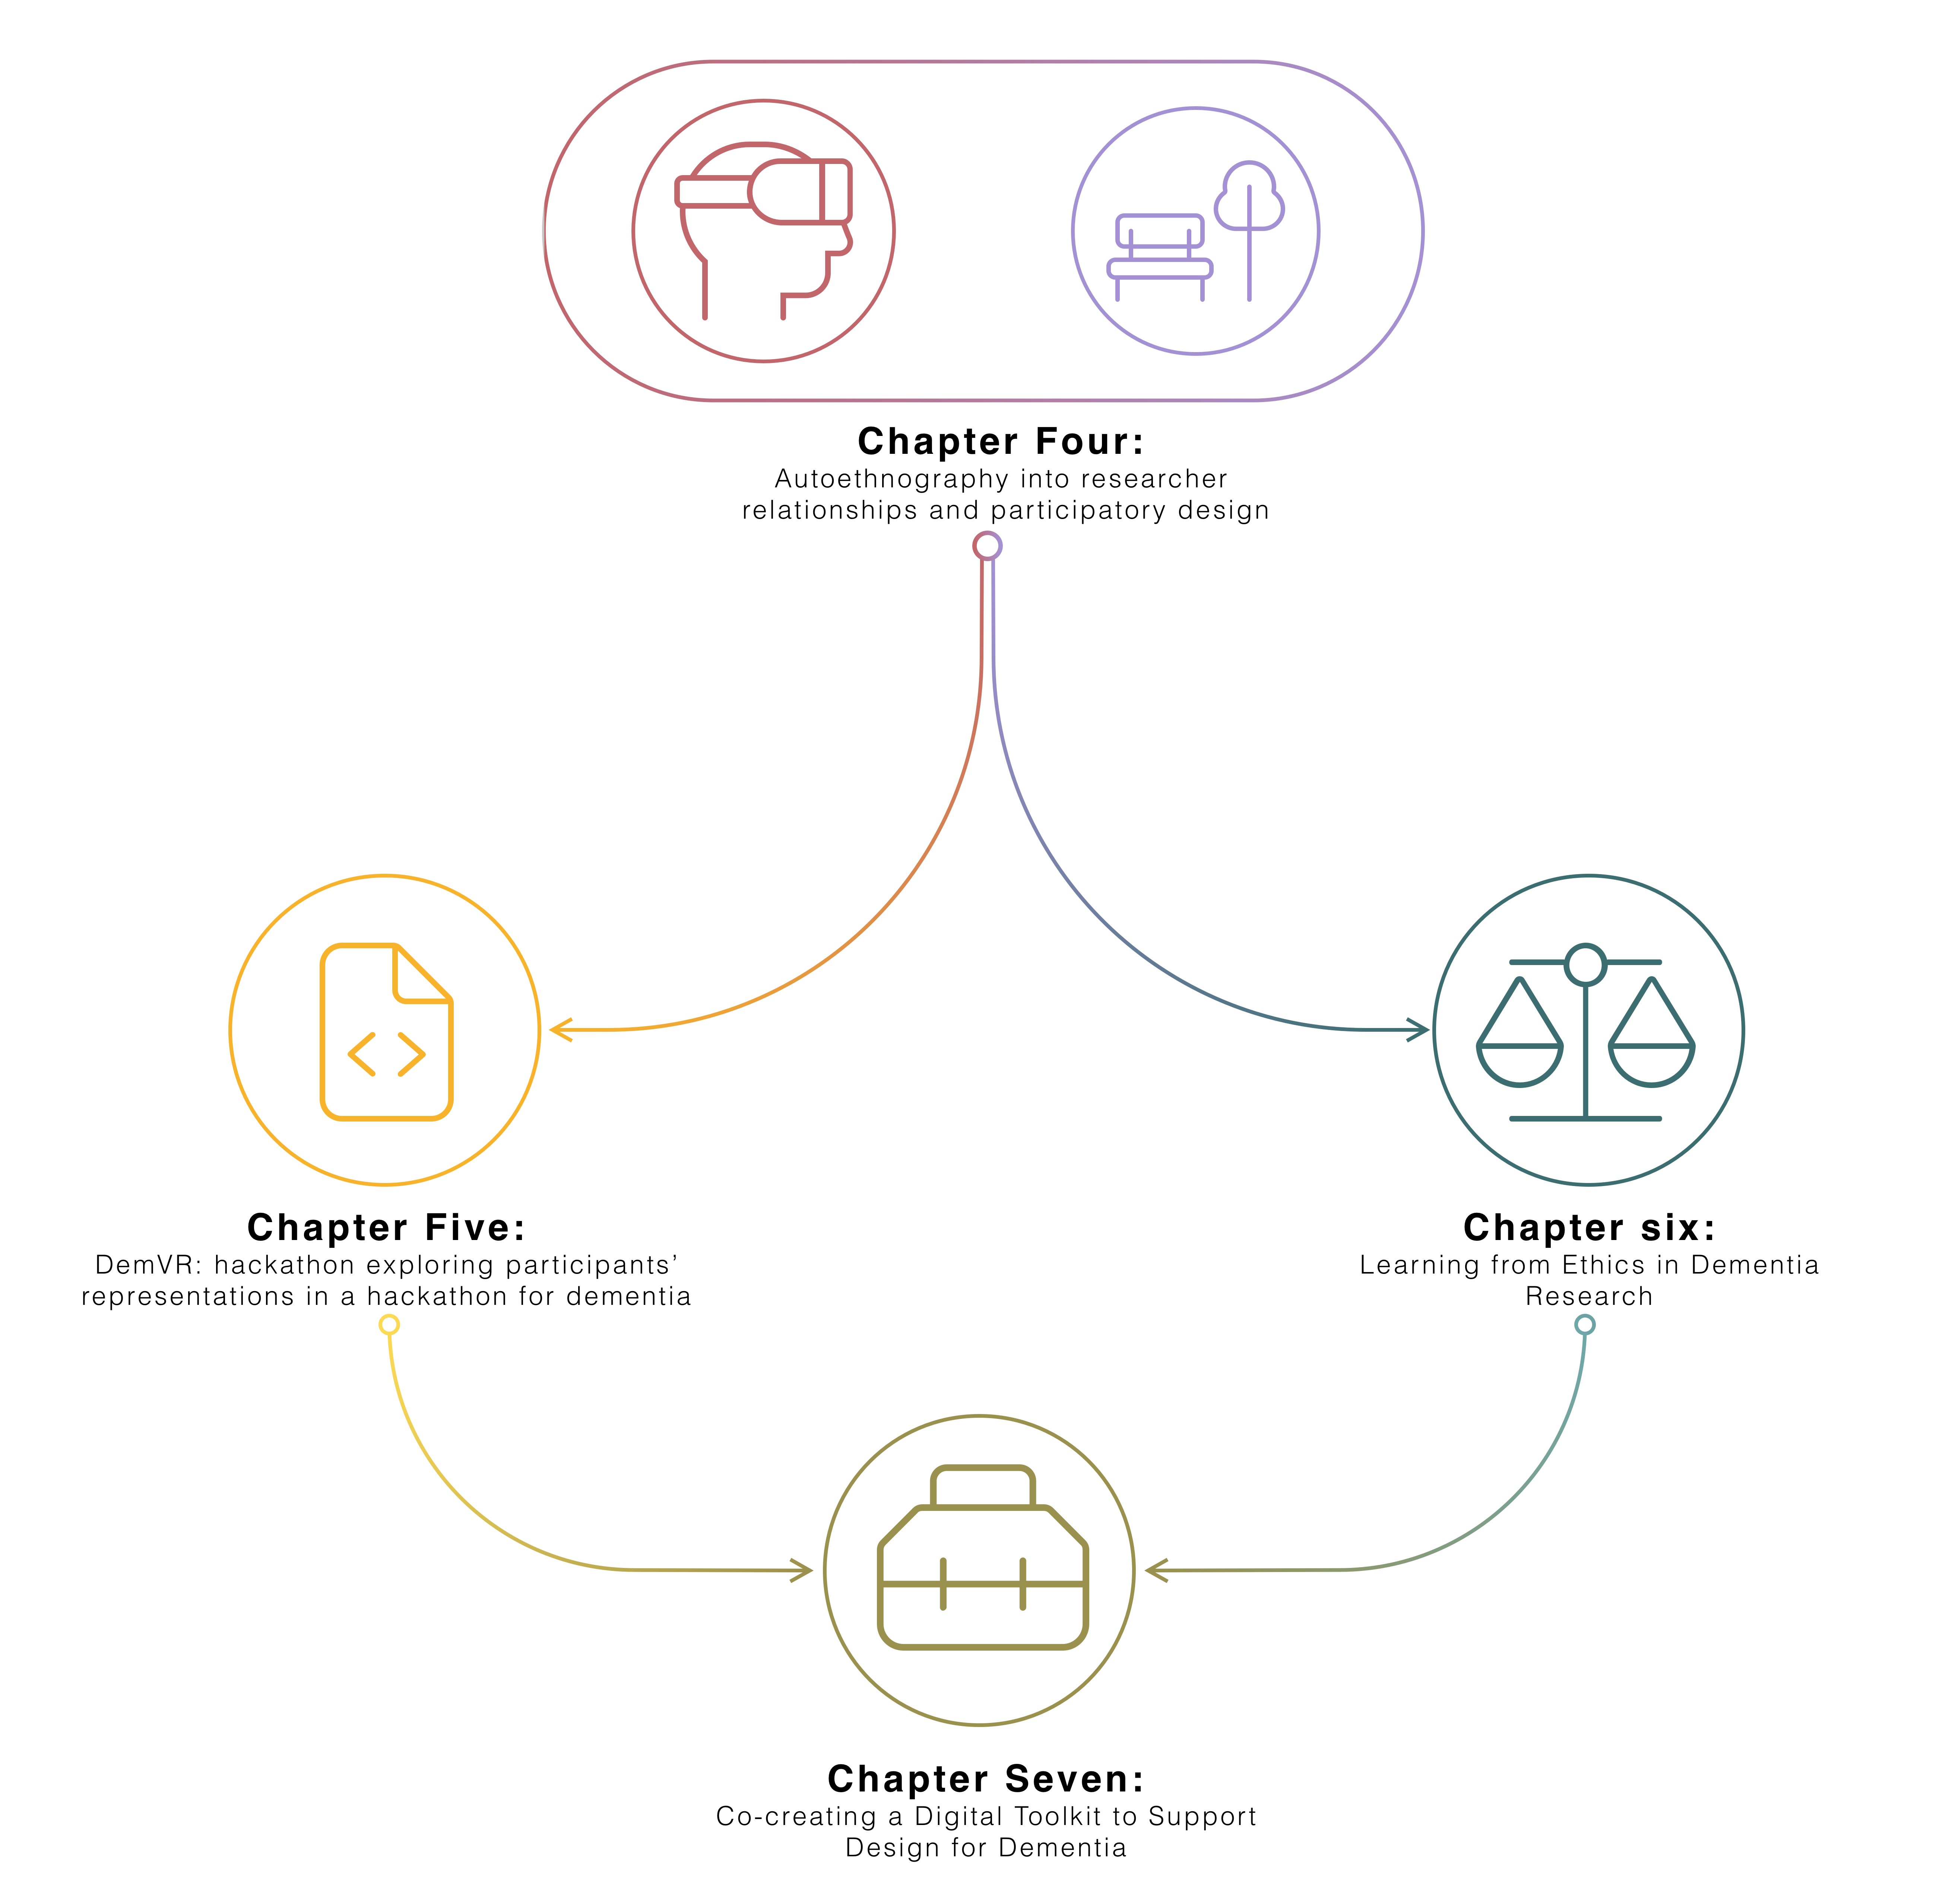
\includegraphics[width=0.6\linewidth]{Images/Thesis_Narrative/Narrative_Full.png}
\caption{Data chapter overview}
\label{fig:Thesis_Overview}
\end{figure}

To tackle these two themes, I organised a hackathon called DemVR to consider how developers/designers and interviewed 22 HCI researchers with dementia experience to examine the complexity of navigating both “everyday” and more formal, institutional ethics in dementia research. Through these two studies, while I have outlined a series of key considerations into my research questions (that I will explore in more detail in the final chapter), the studies have raised numerous questions centred on the ethics of recognising people with dementia in research; the challenges of communication between designers/developers and people with dementia; and how collaboration should be curated for the different groups of people with diverse sets of skills and backgrounds. 

With this in mind, this chapter presents a study working with seven designers, four developers, and five people with dementia who I invited to participate in a three-stage iterative process to explore the type of resources developers and designers need to design with people with dementia and investigate how people with dementia envision their potential participation within a toolkit. Following stages one and two, I used a process of affinity diagramming to help surface a set of design priorities to guide the design for a final dementia design toolkit prototype - which I called the Dialogical Dementia Design (D3) Toolkit. Following our toolkit design, I conducted a final workshop inviting participants to reflect on the prototype toolkit to provide further insights into how designers, developers and people with dementia may contribute, use, and envisage how toolkit components might facilitate co-creation between different groups. Through our inclusive methodology, this paper offers three novel contributions:
\begin{itemize}
    \item  A rich description of a prototype Dementia Toolkit to support designers and developers in co-designing with people with dementia.
    \item  A series of design insights to support toolkit development, including barriers to co-creation, incentives for sustainable participation, and sharing the 'design' role.
    \item A series of directions for HCI and dementia research highlighting how we might balance participants' privacy, safety, and recognition; priorities to contribute and grow a community-owned toolkit; and the accountability and responsibility that designers and developers carry when designing in such sensitive and ever-changing situations.
\end{itemize}

The study covered in this chapter is currently in submission to TOCHI. The study was co-authored by Dr. Kellie Morrissey, and Dr. David Kirk.

\section{Related work}
\label{D3:RelatedWork}
To help ground our work, below I summarise current approaches in HCI to participatory research with marginalised communities, explore priorities and engagement requirements when designing with people with dementia, and review the type of resources and toolkits that have been designed as creativity support for designers and developers. 

\subsection{Representing the experiences and views of marginalised communities in HCI}
\label{RelatedWork:PartOne}
Co-design and participatory design traditions have historically engaged with marginalised communities in order to highlight the agendas and individual needs of members on topics such as rights, benefits, resources, and identity \citep{porter_filtered_2017,scheuerman_safe_2018,devito_social_2019,fraser2000rethinking}. This work has resulted in design practices that examine the acknowledgement of emotion in our research \citep{balaam_emotion_2019}; give careful attention to researcher-participant relationships \citep{clarke_digital_2013}; and create safe spaces to support the sharing of sensitive topics \citep{talhouk_refugees_2016,scheuerman_safe_2018,lazar_safe_2019}. Following this work, the acknowledgement and sensitivity required for participants depends on their desires, needs as a community, and the community’s history that we are building on. Prior work has innovated many of our methodological approaches to better fit our participants: for instance, careful navigation of gatekeeping \citep{sanghera_methodological_2008}, awareness of biases and stereotypes \citep{marsden_stereotypes_2016}, and providing slower, longer-term projects to provide the time to build trust and a relationship between the researcher and participants \citep{foley_care_2019}. Beyond designing for individual needs and desires, working specifically with LGBTQIA*groups \citep{byron_apps_2019}, refugee and immigrant populations \citep{talhouk_syrian_2016}, those with mental illnesses \citep{birbeck_self_2017}, older people \citep{reuter_older_2019}, and reproductive rights advocates \citep{michie_her_2018} has contributed to a more inclusive design that invites \textit{“new ways of doing, making and inhabiting the situation of our world today” (pg.65) \citep{rosner2018critical}}.

This project focused in particular on designing for and with people with dementia, where dementia is a neurodegenerative condition that sees the deterioration of cognitive abilities, often leading to an increased dependence on care, and which can lead to societal stereotyping and stigmatisation \citep{kontos_integrating_2018, benbow_dementia_2012}. Early HCI and dementia work has evolved our understanding of dementia by focusing on the ways in which we involve people with dementia in processes of technology design \citep{lindsay_empathy_2012, suijkerbuijk_active_2019,vines_configuring_2013,wallace_enabling_2012-1}. For instance, \cite{wallace_design-led_2013} use a tailored approach that centred the importance of personhood by paying attention to a person’s individual and unique experiences of dementia to design bespoke digital artifacts for the participants. Similarly, \cite{lindsay_empathy_2012} describes the need for more interpretative data approaches for those at later stages of dementia, which in turn, may require longer-term projects and relationships to form throughout a study. This early work stresses the required need to adapt co-design and participatory approaches to accommodate the differing communication needs of people with dementia, ensuring they are respected rather than infantilised \citep{morrissey_im_2016,muriana2016you}. 

More recent work has seen a critical turn to understanding personhood even in the presence of later stages of dementia, where non-verbal and ambiguous interactions may be more present \citep{dupuis_re-claiming_2016}. \cite{treadaway_sensor_2016} emphasise that recognition and appreciation are crucial even when leaning on tacit, creative activities to support non-verbal interactions. This critical turn is further supported in work by \cite{morrissey_value_2017}, taking an experience-centred approach that shifts the way we see people with dementia-related cognitive deficits as contributing to design choices. While prior work may focus on alleviating a person's cognitive deficit, the critical perspective widens our approach to inclusivity, by celebrating what a person has to offer through more creative and engaging approaches, where those living with a broad spectrum of dementia-related changes can also participate \citep{lazar_critical_2017}.

To help foster empathy with, and understanding of, a person with dementia's experience, there has been a push from dementia activists towards using online interactions and bespoke forums and Twitter to raise awareness and further challenge the stigma surrounding dementia \citep{talbot_how_2020}. \cite{dai2020making} recent work on social sharing through community-based programs describes how future platforms involving people with dementia need to allow flexibility for \textit{"dynamic roles"} where individuals can flip between \textit{"storytellings, listeners, contributors" as the "activities [on the platform] evolve" (pg.10)}. Likewise, \cite{johnson_older_2019} argue that these roles may need support from \textit{"various stakeholders in participating without burdening" (pg.127)} people with dementia. The further involvement of gatekeeping stakeholders may provide useful moderation and provide safety and familiarity on online spaces that can feature bad actors who target the vulnerability of people with dementia. 

This move to online-mediated change-making mirrors a trend in work on participatory platforms and digital civics that has begun examining and developing tools to promote change and support marginalised voices \citep{corbett_exploring_2018}. For instance, \cite{puussaar_making_2018} developed a visual map-based querying tool to provide the public to interpret and understand open-source datasets that are typically incomprehensible by non-professionals. \cite{asad_tap_2017} work on similar civic platforms describes that there is an \textit{"obligation [for] designers and researchers to ensure our work aligns with existing efforts in our respective research communities" (pg. 6314)}. In \cite{foley_student_2020} work on student engagement within dementia care, the authors describe that over time, students started to take \textit{"responsibility for the development of the relationships"} while the person with dementia was \textit{"viewed as experts, with knowledge and stories to share beyond their role as a patient in care" (pg.9)}. However, to support collaboration and engagement between those who are being designed for, and those who are doing the designing, we need further consideration into the articulated needs and desires of such platform users - particularly those within socially complex contexts. 

\subsection{Resources for designers and developers doing participatory HCI work}
\label{RelatedWork:PartTwo}
Much research in HCI has been devoted to the development of toolkits and other creativity support mechanisms, which have variously been used to support design research, creativity, and technological development and implementation \citep{broderick2020theory, ledo2018evaluation}. \cite{ledo2018evaluation} write that toolkits within HCI provide: a) simplifying and fast-track creation, b) assistance in problem-solving processes, c) help to engage new audiences d) help to adapt tools within users workflows and e) support replication to enable scaling. Designers and developers use toolkits to manage collaborative design and \textit{"understand the design situation and the problem at hand and to explore and experiment with potential solutions." (pg.21)\citep{dalsgaard2017instruments}}. For instance, \cite{chen2020interaction} introduce a toolkit for turning conference papers into actionable guidelines and design tips through the curation activity of undergraduate researchers, who review papers and summarise the key findings down into a series of guidelines. Likewise, Tiles, a card-based toolkit for iteratively designing Internet of Things ideas, provides a framework for playful and quick interaction between a small group to support conversation and creative thinking on given design goals and context \citep{mora2017tiles}.

Card sets and games are often employed in such toolkits, particularly as they allow collaboration between multiple stakeholders or members of a team \citep{friedman2012envisioning,culen2015making}.\cite{peters2020toolkits} review of analogue tools note the popularity of card games, as they are helpful to organise ideas, structure activities, spark creativity and heighten playfulness and collaboration. Similarly, \cite{caraban2020nudge} work in developing 'Nudge Deck' supported participants to break their design challenge down into more minor problems and in turn lay out directions for their design. However, the use of design toolkits can face challenges where other cultural contexts and settings interact \citep{peters2020toolkits} , such as when values, goals and technologies displayed on cards may have little to no meaning within the setting. While one approach is to make toolkits more abstract and open to be applicable for different settings, \cite{peters2020toolkits} suggest tools be more \textit{"consciously culturally-tailored" (pg.20) }. This may require involving audiences in the creation and customisation of the tool. Similarly attending to the practical use of such kits, in a recent review of open-source fairness toolkits, Lee and Singh raise a valuable concern, stating creators of such toolkits should\textit{ “remain vigilant to ensure their adoption is aligned to the over-arching goal: to ensure our algorithms reflect our ethical values of non-discrimination of fairness” (pg.12) }\citep{lee2021landscape}. In cases like these, the provision of tools that may be freely used and reshaped by a user community requires further thought about the roles of moderation or expertise, particularly when toolkits may be intended for use or application in marginalised settings. This open-source framing also, interestingly, opens up the possibility that toolkits might move from being static resources (even so far as being printed, boxed and shipped), to being something that evolves and develops over time (a fluid and unfinalisable design tool).

It is clear that creating specialised toolkits for use in particular settings or contexts requires specialist input to ensure the content is appropriate \citep{alshehri2020scenario,meissner2018schnittmuster}. For example, \cite{craig2021development} developed an ethical roadmap for designing at the end-of-life; this roadmap comprised components such as value cards, ‘informedness’ of consent questions, provocations, and value cards to support developers and designers to reflect on and question their approaches to this very contested area of work. To curate the cards and content for the ethical roadmap, the authors worked with a diverse team of experts in end-of-life matters, digital media, and physical object design, as well as with participants whose experiences in bereavement spoke to the toolkit’s use. In a similar study, \cite{shinohara2020design} describe a series of design cycles requiring various stakeholders to develop a set of method cards for social accessibility. While Shinohara emphasises the toolkit should not replace students directly speaking to users, they explain that the toolkit provides \textit{“information about how to interact with expert users” and that this “helped students to know how to start conversations and guide them toward productive discussions” (pg.17:29)}. 

Moreover, during the COVID-19 pandemic, an open-sourced collaborative toolkit known as Covid Creatives Toolkit was curated to support practitioners who needed to migrate their practice to digital spaces quickly \citep{braybrooke2020together}. Initial co-creators of the toolkit quickly realised the resources they offered were leaning towards North American perspectives and needs; they quickly counteracted this by providing an open resource to be maintained by patrons worldwide. This supportive, shared curation for and between diverse backgrounds echoes \cite{lee2021landscape} key finding: that toolkits need to “adapt and integrate to \textit{“plug and play” with the [developers] existing workflow”}. Within this prior work, while toolkits do not replace engaging with the community, they offer expert knowledge for those outside the community to engage and learn about important history and understandings that may be required prior to engagement. Additionally, the breadth of iteration and expert knowledge invested in this work highlights the importance of involving users to contribute to toolkit resources to provide relevant and important information.  

In reviewing the above, I see that many of toolkits have been developed in response to a given problem or design challenge - whether that has been engagement with a particular community, or to provide insight and knowledge on a complex or novel topic. Prior work has highlighted that the content of such toolkits requires careful consideration, and often a set of expert curators to ensure content is ethical and sensitively designed. However, returning to our dementia literature, such work involving people with dementia requires adaptability to ensure inclusive and meaningful engagement. Furthermore, while there are many different types of toolkits that we look to for inspiration for applications within dementia, we must ensure that the toolkits will adapt and fit into the user’s workflow. In turn, this raises the question of what sorts of toolkit interactions we should provide to designers and developers that allow them to collaboratively design with people with dementia. The following section beings to unpack how I approached this challenge. 

\section{Methodology}
\label{D3:Methodology}
Interested in what creativity support designers and developers need to design, for dementia and how people with dementia can be involved in that same process, I invited 11 developers and designers and five people with dementia for a series of workshops and interviews. The following research questions guided the study:
\begin{itemize}
    \item \textbf{Research Question One}: What do designers and developers want and need to know to ethically and sensitively design for dementia?
    \item \textbf{Research Question Two}: How can toolkits and other creativity support toolkits foster dialogical engagement between people with dementia and designers and developers?
    \item \textbf{Research Question Three}: What challenges may arise when shaping a digital toolkit that provides co-creation and curation between designers, developers, and people with dementia?
\end{itemize}

\subsection{Participants \& Online Setting}
\subsubsection{Developers and designers}
Participants were 11 self-identified designers/developers (four women, seven men). I approached recruitment through purposive sampling, ‘\textit{a form of non-probability sampling in which decisions concerning the individuals to be included in the sample are taken by the researcher’}, based upon ‘\textit{criteria which may include specialist knowledge of the research issue’ }(pg.5)\citep{rai2015study}. I recruited through networks which were likely to provide this specialist knowledge, with myself contacting prospective participants from software engineering network in Newcastle; and Dr Kellie Morrissey recruiting through student and graduate network through a local School of Design. Although I believed these to be appropriate groups for the purpose of this research, potential imitations of this approach are detailed in my discussion. 



% this line fixes the vertical padding of text inside the cells
\renewcommand{\arraystretch}{1.4}

% Please add the following required packages to your document preamble:
% \usepackage{graphicx}
\begin{table*}[!ht]
\centering
\caption{Designer and developer demographics}
\label{tab:DeveloperDesignerDemographic}
\begin{tabularx}{\textwidth}{@{} YYYYYY @{}}
\multicolumn{1}{c|}{\textbf{Name}} & \textbf{Age} & \textbf{Gender} & \textbf{Ethnicity} & \textbf{Highest qualification} & \textbf{Professional background} \\ \hline
\multicolumn{6}{c}{\textbf{Designers}}  \\                                                                                      \\
\multicolumn{1}{c|}{\textbf{Conor}}    & 21 & M & White Irish          & Final year 

undergraduate & Product Designer           \\
\multicolumn{1}{c|}{\textbf{Mary}}     & 22 & F & White Irish          & Undergraduate            & Designer                   \\
\multicolumn{1}{c|}{\textbf{Kathleen}} & 20 & F & White Irish          & Final year 

undergraduate & Product Designer           \\
\multicolumn{1}{c|}{\textbf{Sean}}     & 28 & M & White Irish          & Postgraduate             & Designer                   \\
\multicolumn{1}{c|}{\textbf{David}}    & 44 & M & White Irish          & Undergraduate            & Product Designer           \\
\multicolumn{1}{c|}{\textbf{Husainah}} & 20 & F & Irish Moroccan       & Final year 

undergraduate & Product Designer           \\
\multicolumn{1}{c|}{\textbf{John}}     & 22 & M & White Irish          & Undergraduate            & Designer  \\                 \\
\multicolumn{6}{c}{\textbf{Developers}}   \\                                                                                    \\
\multicolumn{1}{c|}{\textbf{Becky}}    & 53 & F & White British        & Postgraduate             & Research Software Engineer \\
\multicolumn{1}{c|}{\textbf{Henry}}    & 25 & M & White British        & Undergraduate            & Software Engineer          \\
\multicolumn{1}{c|}{\textbf{Jay}}      & 29 & M & White Northern Irish & PhD                      & Research Software Engineer \\
\multicolumn{1}{c|}{\textbf{James}}    & 25 & M & White British        & Postgraduate             & Software Developer        
\end{tabularx}
\end{table*}

\subsubsection{People with dementia}
I recruited five people with dementia (one woman, four men) by reaching out to dementia advocacy groups online as well as several dementia networks, asking them to share study information in their weekly newsletters. While I did not receive any interest from network members, three members of the 3 Nations Dementia Working Group committee agreed to participate in the study. With schedule conflicts, not all participants could participate in all three interviews – table \ref{tab:DementiaDemographic} highlights the interviews in which they participated.  

\begin{table*}[!ht]
\centering

\begin{tabularx}{\textwidth}{@{} YYYYYYY @{}}
\textbf{Name} & \textbf{Age} & \textbf{Gender} & \textbf{Ethnicity} & \textbf{Professional Background} & \textbf{Stage of dementia} & \textbf{Interview involvement} \\ \hline
\textbf{Howard} & 58 & M & White British & Healthcare             & Early to middle & 1,2,3 \\
\textbf{Nigel}  & 67 & M & White British & Human rights lawyer    & Early onset     & 2,3   \\
\textbf{Julie}  & 58 & F & White English & Nurse / social worker  & Middle          & 1     \\
\textbf{Masood} & 64 & M & Asian British & Accountant             & Early to middle & 2,3   \\
\textbf{Jim}    & 72 & M & Canadian      & Marketer, communicator & Middle to late  & 1,2,3
\end{tabularx}
\caption{People with dementia demographic}
\label{tab:DementiaDemographic}
\end{table*}

\subsection{Ethics}
Newcastle University Ethical Review Board approved this study. Each participant was emailed an overview of the study and provided with information and consent forms. For the participants with dementia, the I carried out capacity assessment, detailed in the Mental Capacity Act 2005 \citep{oyebode_mental_2005} to verify participants were capable of participating in the study. Following the assessment, each participant provided recorded verbal consent. Each participant was offered to be identified by their real forename or else to be pseudonymised if they preferred. Each participant was offered a £30 voucher (or equivalent) for their contribution.

\subsection{Data collection}
Group workshops with designers and developers and one-to-one interviews with people with dementia were split across three stages of data collection. Stage one and two focused on gathering data to incrementally develop the dementia design toolkit. For the third stage, I presented the toolkit to participants to gather feedback and critique in its roughly ‘final’ stage. Interviews were carried out over Zoom as the preferred choice for participants with dementia. For the workshops, designers and developers joined a scheduled Microsoft Teams’ meeting, with additional activities occurring on a shared online whiteboard space (a \href{https://miro.com}{Miro board}). 

\begin{figure}
\centering
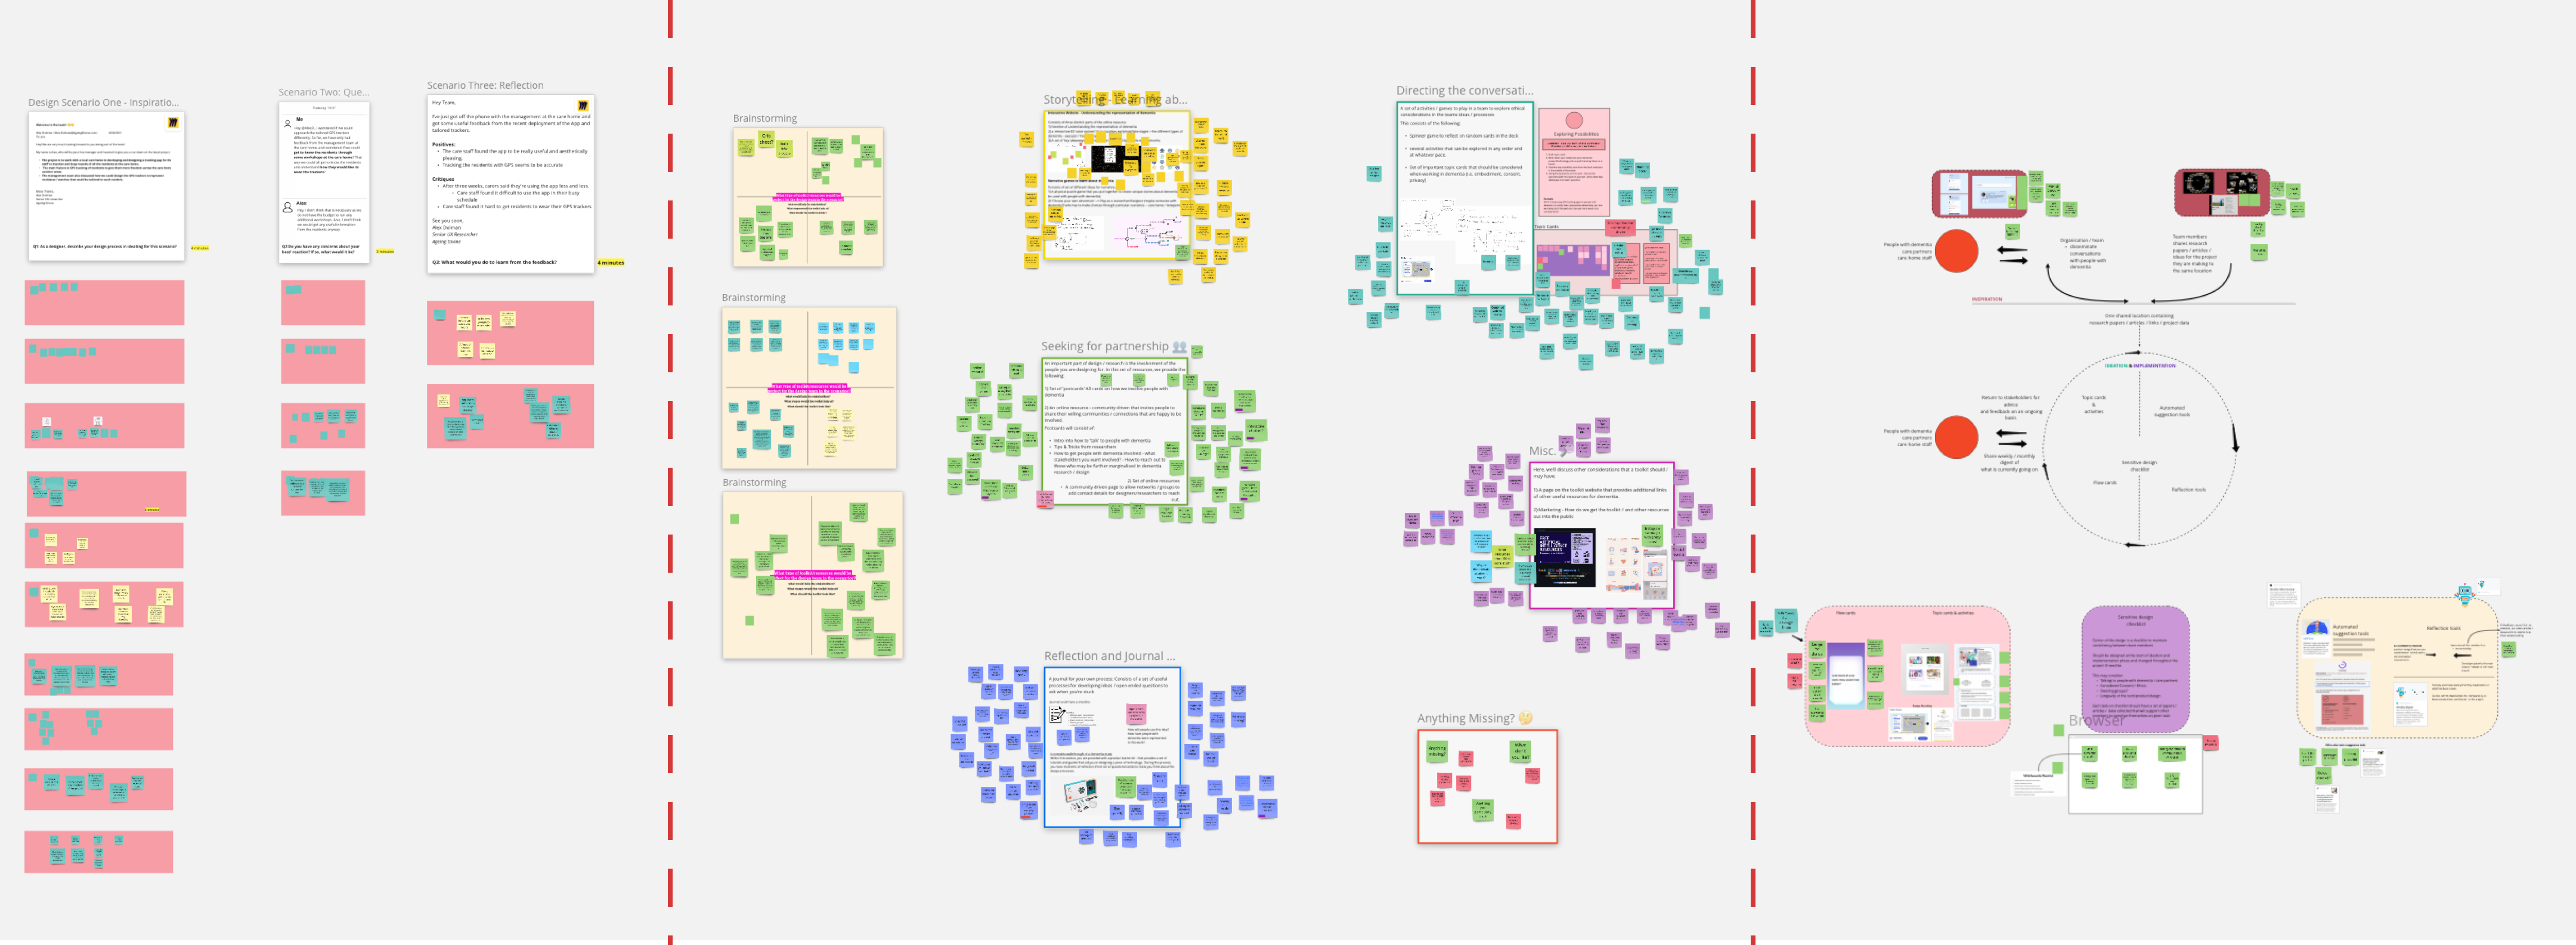
\includegraphics[width=1\linewidth]{Images/D3Toolkit/Fig1.png}
\caption{Stage one, two, and three Miro boards (from left to right)}
\label{fig:StagesD3}
\end{figure}

\subsubsection{Stage one}
In the first workshop, I explored the type of resources that designers and developers use in the creation of new physical and digital artefacts. In discussing toolkits, I conducted an initial walk through of three popular examples – Tiles: IoT \citep{mora2017tiles}, IDEO Method Toolkit \citep{fraga2020inclusive}, and Ethical Explorer Pack \citep{network_ethical_nodate}. Participants then read and responded to design fictions about the work of newly recruited designers/developers for a bespoke care home technology company. The scenarios were intended to provoke questions around early phases of design and development, sensitive conversations within teams, and reflecting on mistakes. The workshop concluded by having a group conversation on \textit{“what type of toolkit/resources would work for the design fiction team?”}.
Interviews with people with dementia in stage one used open-ended questions and prompts to explore: 1) important topics in dementia, 2) experiences with working with designers/developers, 3) involvement of people with dementia, 4) public engagement with dementia, 5) storytelling in dementia, and 6) dissemination of dementia knowledge for learning.
From the initial workshops and interviews, I began to cluster the conversations using affinity diagramming – a well-recognised early-stage design process for organising ideas and opinions into groups based on their relationship to one another \citep{lucero2015using}. 



\subsubsection{Stage Two}
\begin{figure}[h]
\centering
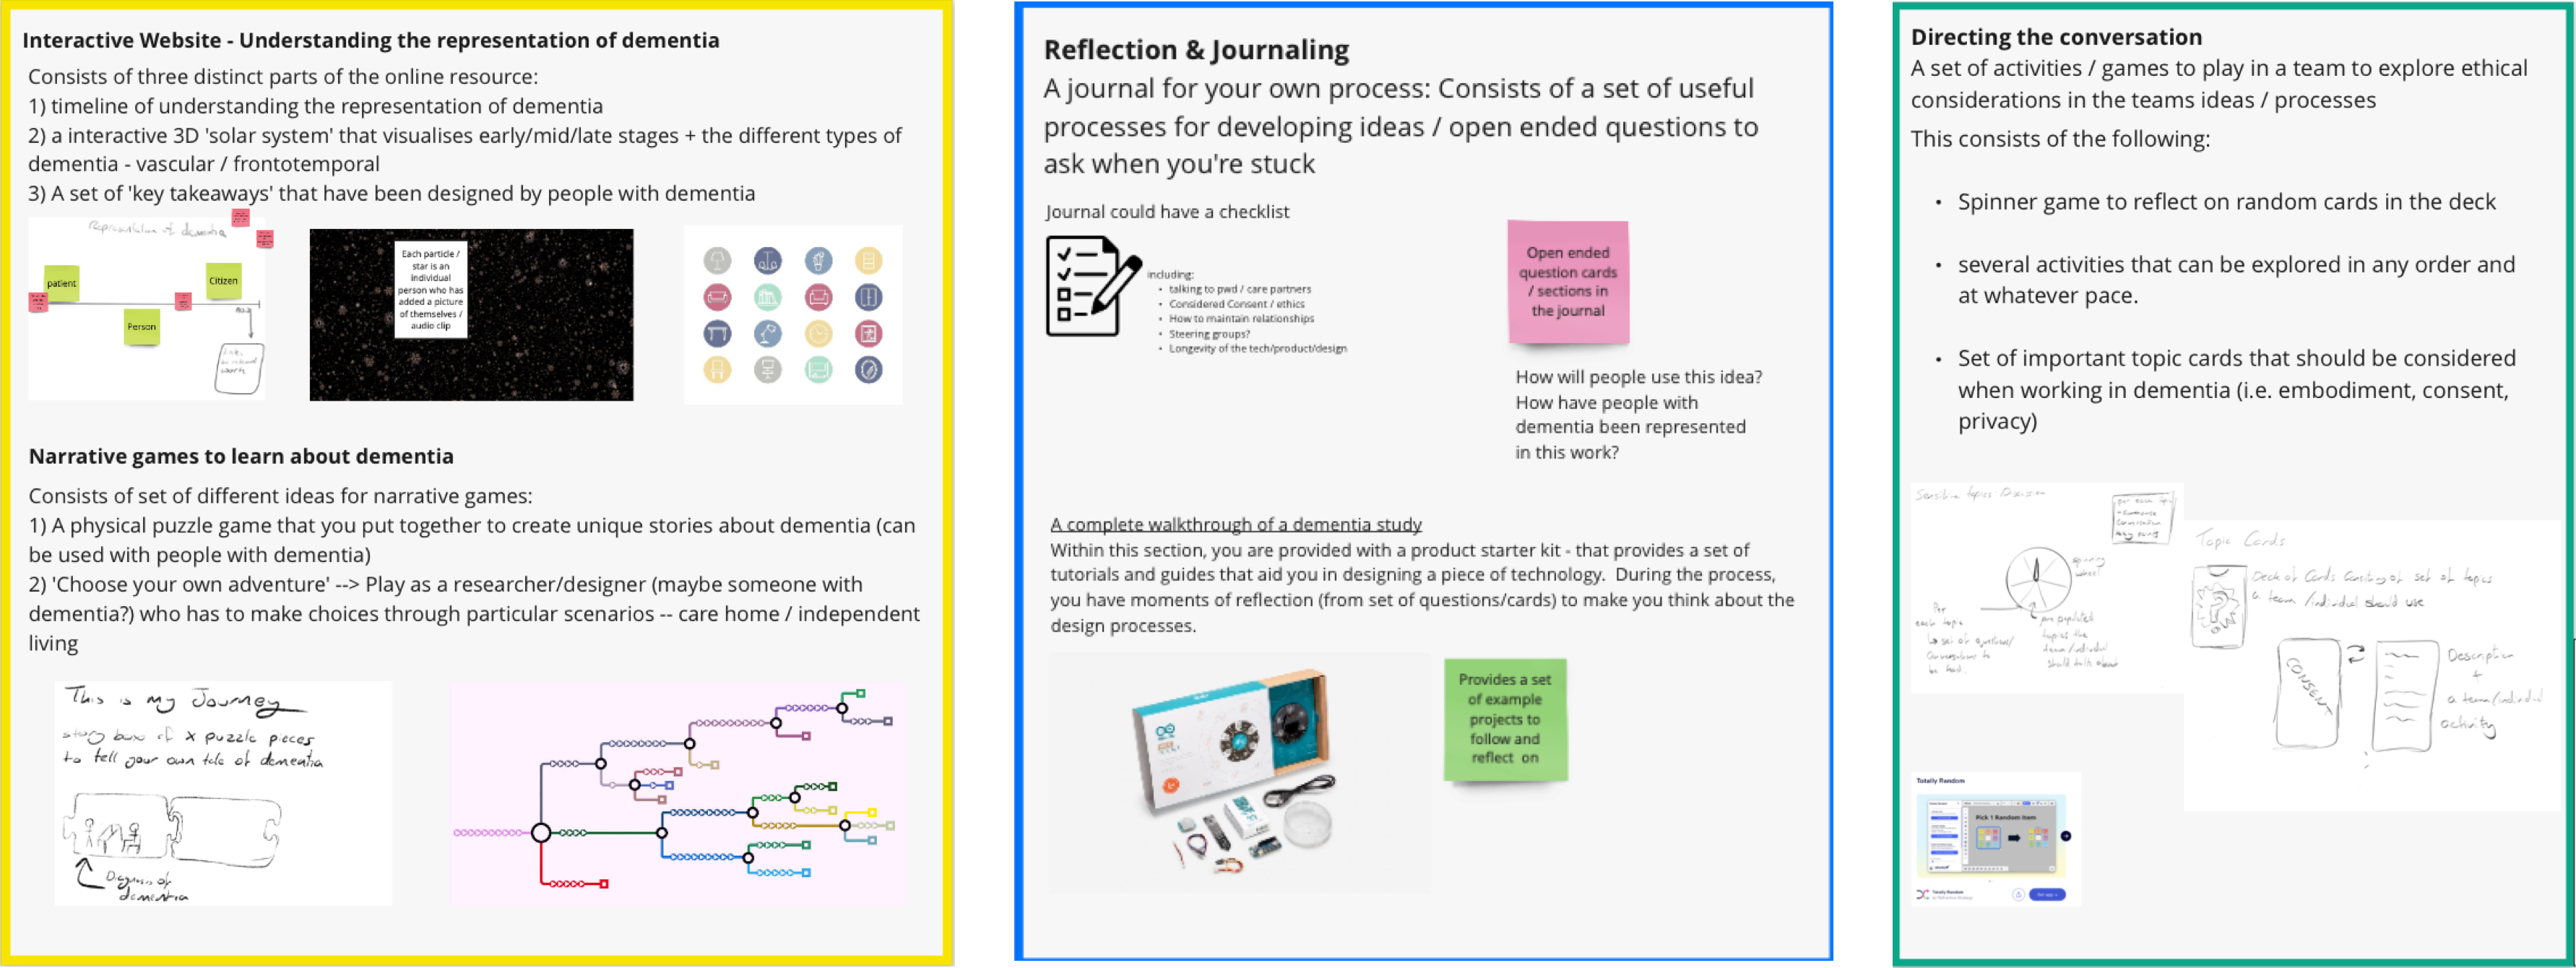
\includegraphics[width=1\linewidth]{Images/D3Toolkit/Fig2.png}
\caption{Stage Two Category Examples: storytelling about dementia, reflection, and journaling, and directing the conversation (left-right)}
\label{fig:StageTwoDesigns}
\end{figure}
In stage two, research engagements explored ten ideas which emerged via the process of affinity diagramming. The ten ideas were categorised into the following categories: 1) storytelling and learning about dementia, 2) seeking partnership, 3) reflection \& journaling, 4) directing the conversation, and 5) community-driven toolkits. During the workshop and interviews, the first author walked through each category and facilitated conversations around topics, preferences, and participants’ workflows. Concerns regarding dementia representation within the toolkit and the involvement of people with dementia were discussed in interviews with people with dementia. Returning to our affinity diagram, I then added our stage two data to the diagram and grouped all the data into a more articulated set of design rationales, described in detail in section \ref{D3:Rationale}.


\subsubsection{Stage Three}
\begin{figure}[h]
\centering
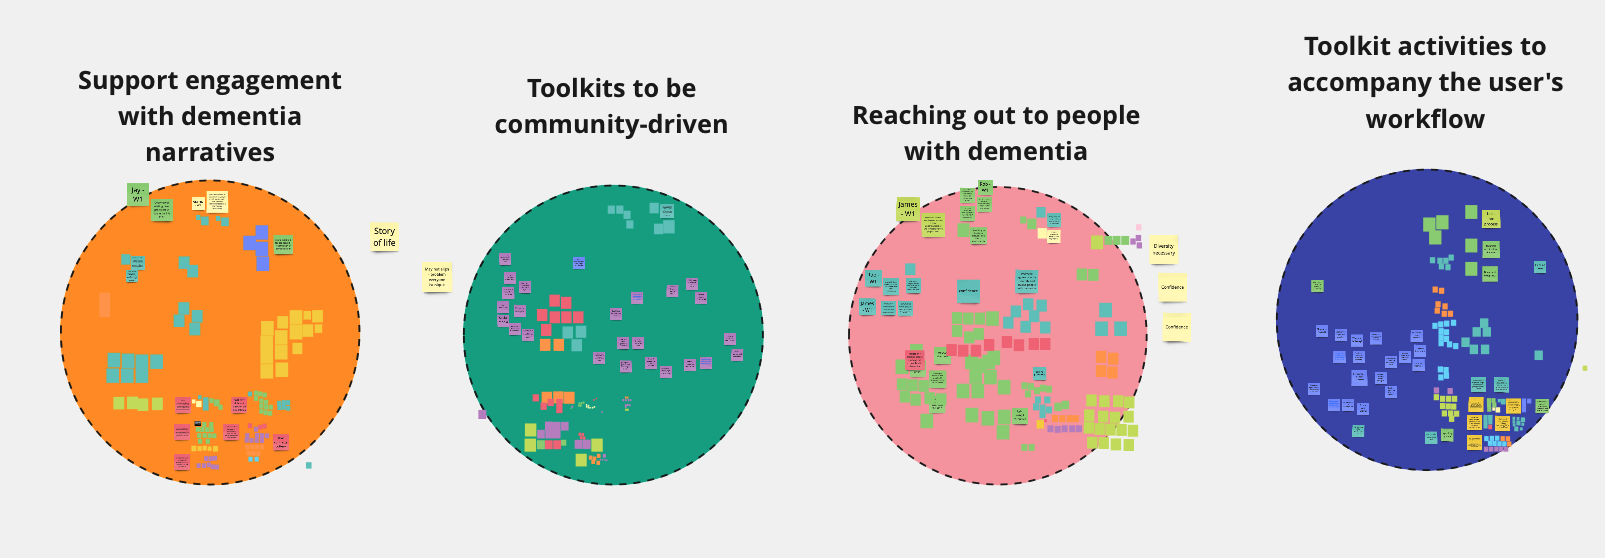
\includegraphics[width=1\linewidth]{Images/D3Toolkit/Fig3.png}
\caption{Final Affinity Diagram for our design rationale}
\label{fig:AffinityDiagram}
\end{figure}

Finally, in stage three, I presented a prototyped (via on-screen mock-ups) toolkit consisting of resources to assist participants in the design of technologies for and with people with dementia. In this engagement, I presented the individual components of the toolkit (described in section 5) with prompts to elicit further discussion, i.e.,\textit{ “what type of privacy concerns should this component consider?”}, and \textit{“how could you see this component benefitting you in ideating new design responses?”}. 

\subsection{Data and Analysis}
I gathered data in the following ways: a) Microsoft Team’s built-in recording and transcription tool for workshops with designers and developers, and b) Google Pixel on-device Audio Recorder that supports offline text to speech for translation for interview with people with dementia. I then revised both the video and audio recordings’ auto-transcriptions for any misinterpretations by the auto-transcription models \citep{bokhove2018automated}. Data collection consisted of eight designer and four developer workshops, and 11 interviews with people with dementia. Breakdown of data can be seen below in table \ref{tab:D3-dataCollection}. For signposting where quotes come from, our findings use the abbreviation seen in table \ref{tab:D3-dataCollection}.

\begin{table*}[!ht]
\centering
\caption{Data Collection (audio)}
\label{tab:D3-dataCollection}
\begin{tabularx}{\textwidth}{@{} YYYYY @{}}
\textbf{Participants \& abbreviation}                        & \textbf{Stage one} & \textbf{Stage two} & \textbf{Stage three} & \textbf{Total}       \\ \hline
People with dementia interviews \textit{(interview\{1,2,3\})} & 227 minutes & 317 minutes & 309 minutes & \textbf{853 minutes} \\
Designer workshops \textit{(W\{1,2,3\} - Designer)}   & 170 minutes        & 175 minutes        & 173 minutes          & \textbf{518 minutes} \\
Developer workshops \textit{(W\{1,2,3\} – Developer)} & 62 minutes         & 123 minutes        & 56 minutes           & \textbf{241 minutes}
\end{tabularx}
\end{table*}

My analytical approach followed a Thematic Analysis (TA) in line with the instructions set out by  \cite{braun_using_2006,braun_one_2020}. This process consists of seven steps. The first step is to prepare transcripts. Second,  I familiarised themselves with the data by reading and interpreting the data while referring to the research questions. Following, I ordered the data from stage three onto a Miro Board to make sense of the similar conversations between the different groups. This helped to explore what topics resonated between the groups, and what topics were unique to the individual groups. Third, I moved onto the coding process to identify all relevant data by reviewing each quote, tagging, and highlighting anything of interest. In the fourth and fifth steps, the I organised codes into potential linking themes across the participants. By the sixth step, the I had weekly meetings with my supervisors to discuss if initial themes fit the original research questions and constructed and defined and named the themes. Finally, the seventh step is developing and writing the analysis presented in section \ref{D3:Reflections}.

\section{Developing a design rationale for dementia design toolkit}
\label{D3:Rationale}
This section, drawing from data in stages one and two, details the results from our initial affinity diagramming process which helped to shape an early design rationale and inform initial toolkit components.

\subsection{Empathy and appreciation for a diversity of experiences}
Designers and developers expressed interest in reading and listening narrative about dementia as a way of learning and contributed ideas about how a toolkit may incorporate this – for instance, Kathleen suggested a \textit{“VR simulation of a walk through a day in the life of dementia” (W2 – Designer)}. However, Jim, who is living with dementia, argued that such a simulation may give a \textit{“warped sense of dementia” (interview1)}. This criticism helped to decide that simulations like these may not be appropriate for our toolkit; instead, designer Sean spoke about a wish to learn about \textit{“spectrum of dementia to know how to design for different stages” (W2 - Designer)}. This aligned with Howard (participant with dementia), who affirmed that \textit{“everybody’s experience [of dementia] are different” (interview1)}. Julie, also living with dementia, argued that designers and developers must be aware of the differing experiences of ‘living well’ and the often life-changing difficulties that come along with dementia. Working from this data in a process of affinity diagramming, I note the following design needs:
\begin{itemize}
    \item A way to quickly grasp the changing nature through exploring stories clustered by theme or diagnosis.
    \item For stories of dementia to portray ‘living well’ as well as challenges of dementia through a range of media formats.
\end{itemize}

\subsection{Putting dementia into dialogue with design}
From our workshops, participants generally believed that people with dementia should somehow be involved in the design process if they were to later become users of a design artefact. Howard argued that \textit{"people with dementia should be involved from the very beginning [of the project]" (interview1)}, with Julie agreeing that it’s "\textit{best way to learn about dementia" (interview1)}. However, designers and developers described \textit{“a lack of confidence to talk to people with dementia” (W2 – Conor/Designer)}. While communicative abilities can change as dementia progresses, Julie describes being mindful that talking to people with dementia is simply \textit{“being human… just be yourself. Speak to us like humans" (interview2)}.
The designers and developers suggested the toolkit could provide a set of resources to \textit{"feel reassured... and have a confidence booster" (W2 – David/Designer)} when reaching out to people with dementia. Participants suggested that these resources could be guidelines or \textit{"prep cards" (W2 - Henry/Developer)} developed by researchers and people with dementia to help to \textit{"normalise and provide some ‘dementia 101’ to establish the basics" (interview1 - Jim)}. Participants also raised the idea of having a database of people with dementia who are happy to be contacted about involvement in design studies. Husainah wished to \textit{"[know] a bit of information on the person in the shared network" (W2 - Designer)}, which in turn would help to a) know if they are interested in your design artefact/process and b) help with \textit{"starting a conversation on interests or who they are" (W2 - Designer)}.
Reinforcing a general wish to learn from people with dementia, Kathleen also suggested that \textit{"designers [could] submit questions [to the resource] that people with dementia would answer" (W2 - Designer)}, and Howard suggested \textit{"sending videos to [dementia] groups, which would facilitate the recordings or written replies which may help to include those who can't use technology" (Interview2)}. Again, working from this data in a process of affinity diagramming, I note the following design needs:
\begin{itemize}
\item The sensitive and ongoing creation of resources to proactively prepare designers and developers to contact people with dementia in a way which recognizes the changing nature of dementia. 
\item A way for safe and comfortable dialogical interactions to be invited, and then occur, between designers, developers, and people with dementia.
\item A forum or process for designers and developers to propose questions for people with dementia to answer.
\end{itemize}

\subsection{Integrating with existing workflows}
Participants were curious about how creativity resources might be incorporated into their existing workflows. Kathleen indicated resources \textit{"would be helpful during the ideation and research stage" (W1- Designer)}, while Husainah stated that resources \textit{"should not be too restrictive" because "designers design in different ways" (W1 - Designer)}. All designers and developers generally preferred to move away from material toolkits, preferring \textit{"apps or a website to replace physical [activities]”}. 
Another universal preference was for a series of checklists to provide helpful scaffolding processes or tips when designing for dementia. David said that such checklists \textit{"make sure not to leave out the important topics" (W2 - Designer)} and provide confidence in \textit{"knowing the checklist suggestions are guidance from experts [in the field] who know what requirements you may want to consider" (W2 - Designer)}. In the developer workshops, Henry described the difficulties of getting a team to \textit{"reflect on and document decisions made within the team" (W1 - Developer)}. Still, he acknowledged that a set of \textit{"blueprints"} or \textit{"checklists"} may make it easier to \textit{"get teams to talk about sensitive topics" (W1 – Developer)}. 
While critical thinking questions were well received by designers, developers Henry and Jay raised concerns that team activities are \textit{"too time-consuming" (W2 - Developer)}, and in particular, pausing a workflow to engage in a structured card activity may be disruptive. Inspired by the data, I moved forward to try to incorporate the following design needs:
\begin{itemize}
\item Toolkits must fit into the designer or developer’s workflow	
\item Toolkit resources should aim to provide reflection and critical thinking
\item Resources must be able to be digital rather than physical (at least in this instantiation)
\item Design tools could vary across stages of the design/development process 
\end{itemize}

\subsection{A collaborative and unfinalisable toolkit}
Developers expressed an interest in contributing on an ongoing basis to the set of resources if it was an open-source project; and people with dementia similarly described a wish to contribute regularly, with Nigel stating that he could offer insights within such an arrangement, resulting in \textit{“a bubble of people bouncing ideas off each other” (interview2)}. Julie’s interview supported this – she envisioned how people with dementia might highlight issues with \textit{“technical terms, abbreviations” (interview1)} or \textit{“alter stigma, stereotype related content”}. Howard cautioned however that such involvement of people with dementia would require significant attention to accessibility to not feel \textit{“disempowered to engage with the material if [you] have to be assisted by others” (interview2)}. 
All participants supported a general view that moderation and guidance in maintaining relevant and quality content is required. Husainah argues that, although sharing resources is useful, \textit{"custom made resources are more helpful as they are less overwhelming” (W2 – Designer)} and raises an essential concern that community shared resources can often become overwhelming and lack structure if no moderation structure is in place. Jay suggested a structure for narrowing down content with concentrated framing similar to \textit{"Github Awesome Lists” (W2 – Developer) }\citep{sorhus_sindresorhusawesome_2021}. Additionally, blueprints for resource components, which aim to plan and scaffold content material, could offer a structured process for community contribution.
Our data within this category points to the follow design priorities:

\begin{itemize}
\item Put in place a structure which allows a toolkit to be updated by a community of designers, developers, and people with dementia
\item Design processes that scaffold and structure the creation of community-added content in order to maintain consistency through moderation and blueprints
\item Consider how such contributing processes could be made accessible and transparent to ensure the comfortable engagement of people with dementia
\end{itemize}

\section{Dialogical Dementia Design (D3) Toolkit}
\label{D3:Toolit}

\begin{figure}[h]
\centering
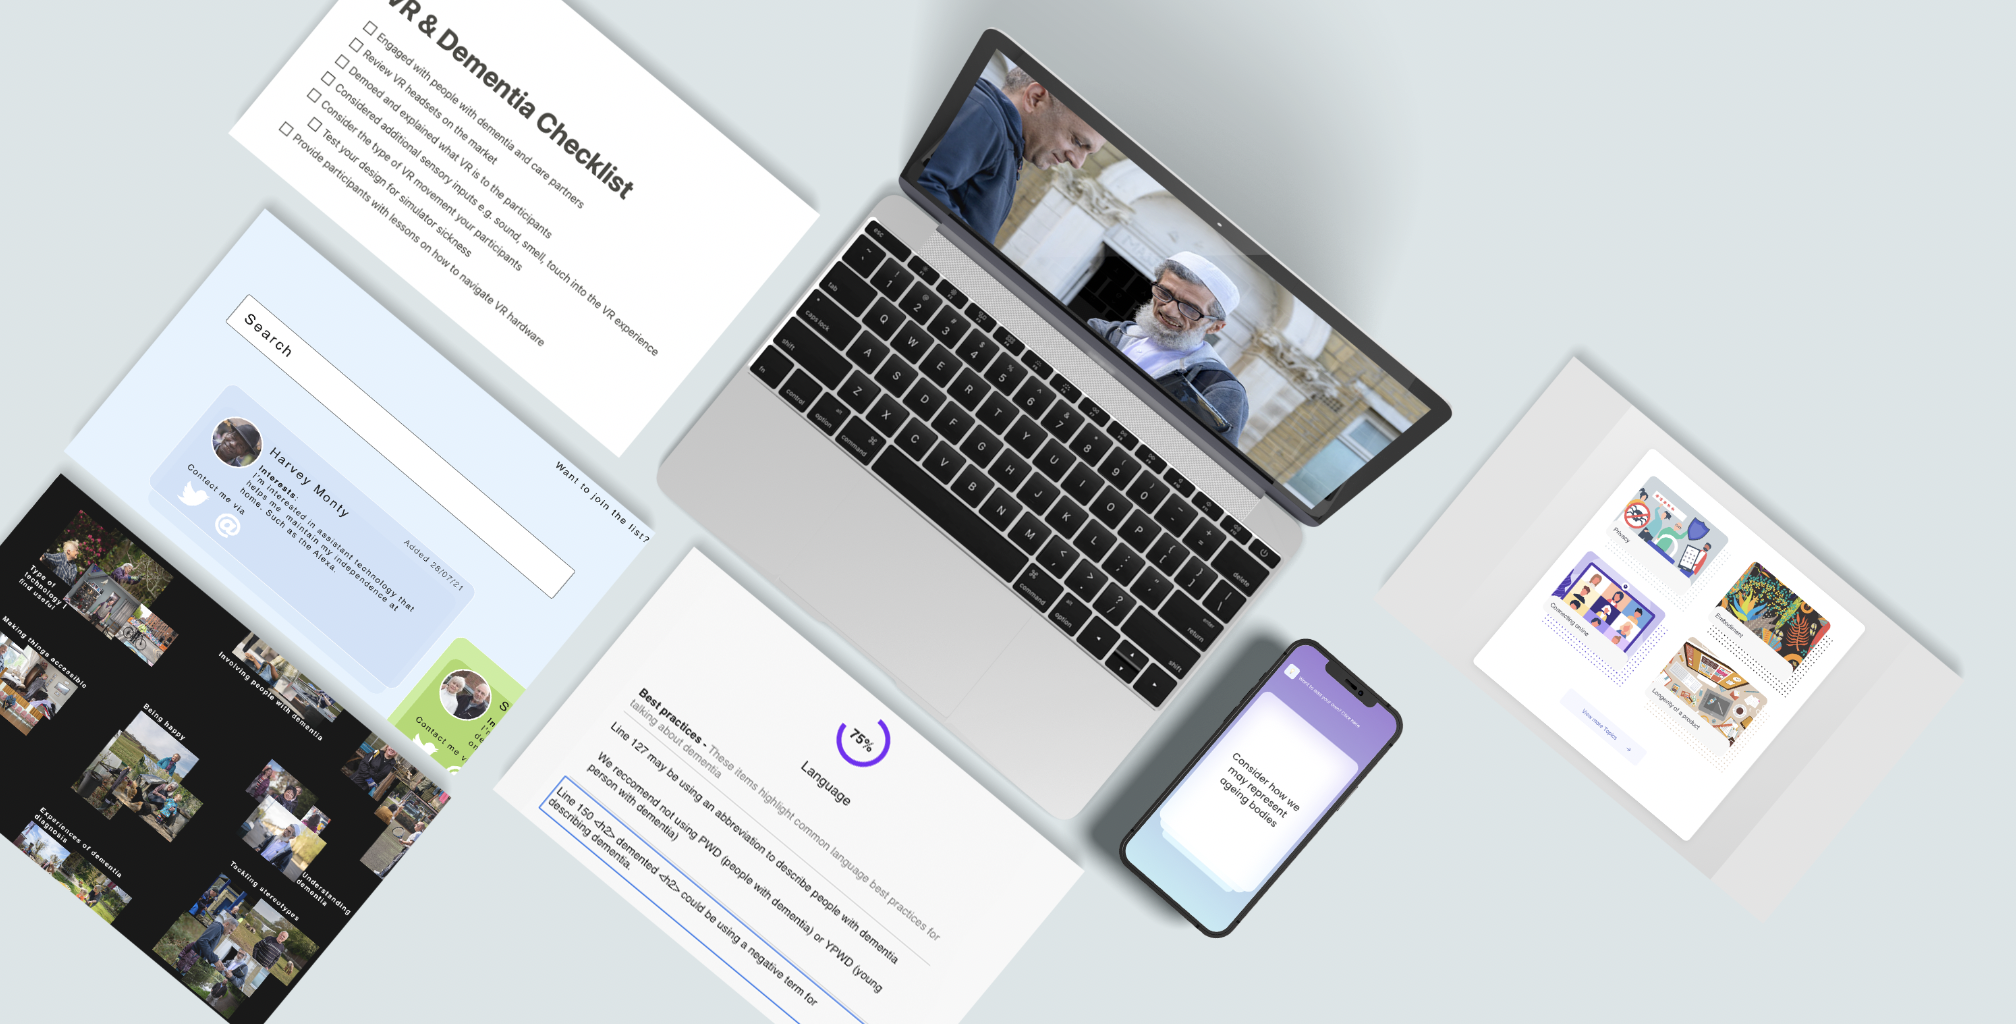
\includegraphics[width=1\linewidth]{Images/D3Toolkit/Fig4.png}
\caption{Different components that create D3 Toolkit}
\label{fig:D3Overview}
\end{figure}
Based on the data collection and affinity diagramming, I created a detailed mock-up prototype of what a dialogical dementia design toolkit may look and feel like and the processes it might support, based on participants’ wishes and preferences. In this section, I describe the individual components of the Dialogical Dementia Design (D3) toolkit. The toolkit is a set of resources to help designers and developers in the ideation, inspiration, and implementation phases of their work with people with dementia. Furthermore, it offers several pipelines for people with dementia to contribute to the individual resources, further described in the individual component descriptions. The phases are as follows:

\begin{itemize}
    \item 
\textbf{Inspiration phase}: Based on our participants’ descriptions of their work patterns, here the inspiration phase is about gaining a fuller understanding about the topic at hand. Our toolkit provides three inspiration components to assist in learning about, and reaching out to, people with dementia, while supporting organised design thought and documentation processes. These three components are:
\begin{itemize}
    \item \textbf{Our Shared Story }– A website for publicly-shared stories from people with dementia grouped into topics and themes to illustrate the diversity of experiences within dementia, as well as their ever-changing nature.
    \item \textbf{Dementia Friends} – A web page consisting of profiles of people with dementia who are interested in research involvement. 
    \item \textbf{Foresight Checklist }– A shared set of community-created checklists to provide suggestions and steps for designers and developers who are navigating the complexity of technology and dementia.
\end{itemize}
\end{itemize}

\begin{itemize}
    \item \textbf{Ideation phase}: Our resources in this phase focus on providing users with ways to generate ideas or identify design opportunities that they may initially discounted over. These components are the following:
    \begin{itemize}
        \item \textbf{Flow Cards} – A set of quick idea cards that orient users towards often-ignored capabilities or communication modalities in dementia; these would be organised via a web-app, for designers or developers to use when they hit a creative block. For example, \textit{“pay attention to non-verbal interactions”}.
        \item \textbf{Guiding Topic Cards} – series of detailed cards focused on relevant topics in technology and co-design with people with dementia. For instance, designers and developers may need to know about legal and care frameworks for ascertaining capacity for consent; or take account of privacy requirements for designing technology with people with dementia.
    \end{itemize}
\end{itemize}

\begin{itemize}
    \item \textbf{Implementation phase}: This phase supports the later stages of artefact/system development, providing feedback and suggestions based on community-contributed ‘best practices’: 
    \begin{itemize}
        \item \textbf{Suggestive Guidance pack} – A automated tool to be run on a website or other system/artefact to provide guidance by comparing text, images, and other media to dementia best practices. 
    \end{itemize}
\end{itemize}

The following sections describe a breakdown of each component and how collaboration between designers, developers and people with dementia may look when using our toolkit. 

\subsection{Inspiration phase}
\subsubsection{Our Shared Story}

\begin{figure}[h]
\centering
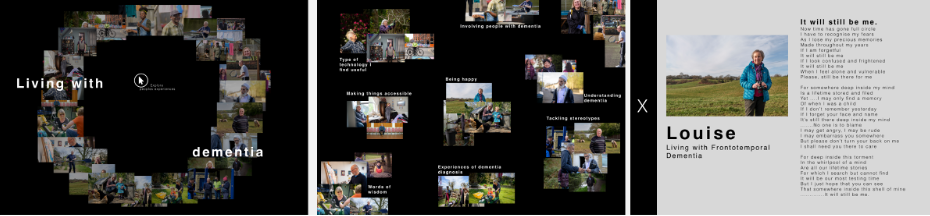
\includegraphics[width=1\linewidth]{Images/D3Toolkit/Fig5.png}
\caption{Navigating Our Shared Story page}
\label{fig:OurSharedStory}
\end{figure}
Our Shared Story allows people with dementia could share their diverse and often in-flux stories via audio, video, or text. Through this medium, the tool will tag and map the experiences of individual people together to support designers and developers in a) exploring diverse participants’ experiences of similar challenges or opportunities, and b) to map the trajectories of dementia to understand the different challenges people may have at different stages of the condition. Provoking insight into the changing nature of dementia, the website provides the user with suggested stories related to the previous story they were reading, which may for instance relating to topics and diagnoses; or else more granular experiences. Such a tool will allow for a variety of experiences to be expressed in their individuality (rather than aggregating them quantitatively), welcoming narratives of dementia which are focused around ‘living well’ but also allowing participants to discuss their challenges. Within this framework, participants can propose questions for other community members to answer, thus supporting the ongoing creation of new narrative threads. 

\subsubsection{Dementia Friends}
\begin{figure}[h]
\centering
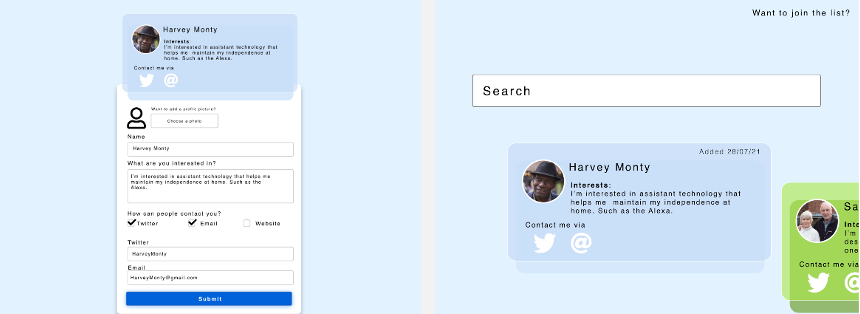
\includegraphics[width=1\linewidth]{Images/D3Toolkit/Fig6.png}
\caption{Platform for 'Dementia Friends'}
\label{fig:DementiaFriends}
\end{figure}
Participants expressed concern about not knowing where to start in reaching out to people with dementia, despite participants living with dementia in general welcoming engagement with designers and developers. Dementia Friends is a portal where people with dementia are asked to share their name, interest, and contact details (Twitter, Facebook, Email) via a form that connects to a database. Upon submission, designers and developers will then be able to search (based on the interests) and contact the different signed-up members to find potential participants for their research. Furthermore, signed-up members are provided with yearly on-going consent check-ins to remind them of this resource, and ask if they would like to continue to be part of the database.

\subsubsection{Foresight Checklist}
\begin{figure}[h]
\centering
\includegraphics[width=1\linewidth]{Images/D3Toolkit/Fig7.png}
\caption{Foresight checklist example on VR and dementia}
\label{fig:ForesightChecklist}
\end{figure}
Participants sought tools to help them ‘check’ their work to ensure it is incorporating best practice guidelines within the particular area. Within this section of the website, the public may share their suggested checklists for each new project, based on prior work. For instance, a researcher who has previously worked in VR and dementia may submit a set of suggestions that they found helpful (seen in figure \ref{fig:ForesightChecklist}).

\subsection{Ideation phase}
\subsubsection{Flow cards}
\begin{figure}[h]
\centering
\includegraphics[width=1\linewidth]{Images/D3Toolkit/Fig8.png}
\caption{Flow cards}
\label{fig:FlowCards}
\end{figure}
Our Flow cards aim to promote creativity during a creative block in the process. As a starting point, I envision these cards as consisting of 100 questions formulated by researchers and people with dementia, such as \textit{“pay attention to the non-verbal”}, \textit{“explore how you can support an individual’s choice”}, and \textit{“consider how we represent ageing bodies”}. Users will find the cards on a webapp and will swipe or tap the screen to explore the different cards that are randomly sorted. Users will also be able to offer additions to these pre-made questions. 

\subsubsection{Guiding topic cards}
\begin{figure}[h]
\centering
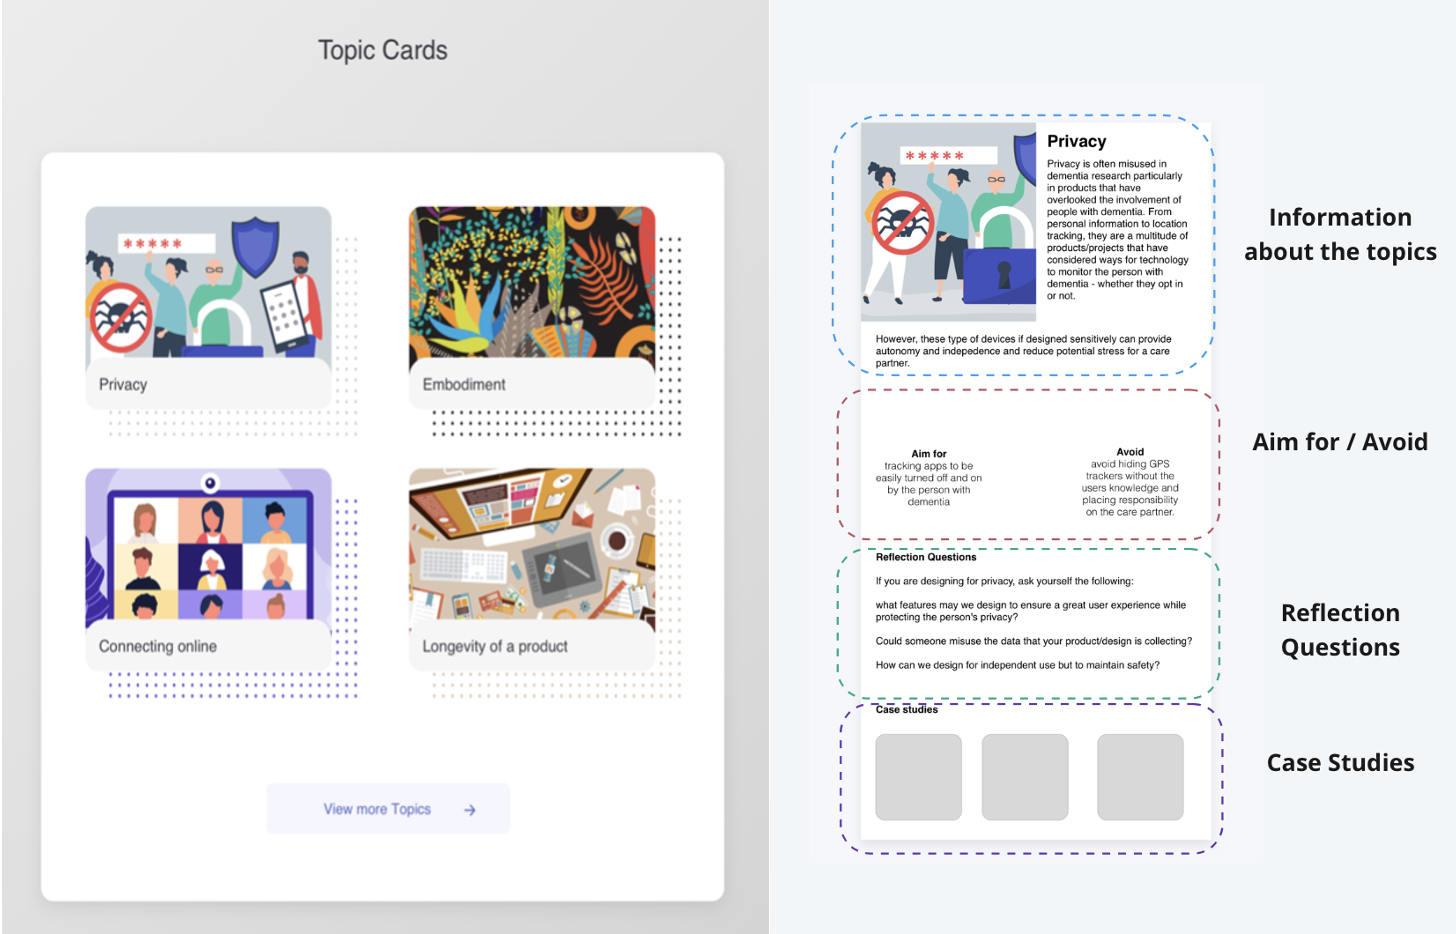
\includegraphics[width=1\linewidth]{Images/D3Toolkit/Fig9.png}
\caption{Guiding topic cards (blueprint design on the right)}
\label{fig:topicCards}
\end{figure}
Participants wanted tailored yet concise knowledge around technology and dementia provided by those with expert experience. In our toolkit, we envision this content as a set of individual topic cards that designers and developers could use to reflect on when working. For example, a guiding topic card may provide information on cognitive changes in dementia when designing interfaces or avoiding perceptual problems in dementia when creating digital assets. To maintain consistency and quality of the cards, I also envision the provision a blueprint that users must follow when creating a new topic card, which must contain:
\begin{itemize}
    \item \textbf{Information about the topic}: paragraph describing the topic in relation to dementia.
    \item \textbf{Aim for / Avoid}: a set of dos and don’ts for that topic. For example, in the privacy example above: Aim for – tracking apps to be turned off by default and Avoid – hiding GPS trackers without the user’s knowledge. 
    \item \textbf{Reflection questions}: Questions for designers and developers to reflect upon in refining their design concepts. For instance,\textit{ “How can we design for independent use while balancing maintain safety?”}
    \item \textbf{Case studies}: A section for the curator to add additional links to relevant articles or projects. For example, in the perceptual problems example above, a case study may focus on non-repeating patterns in fabric and textile development.
\end{itemize}

\subsection{Implementation phase}
\subsubsection{Suggestive guidance pack}
\begin{figure}[h]
\centering
\includegraphics[width=1\linewidth]{Images/D3Toolkit/Fig10.png}
\caption{Suggestive guidance pack to reflect on best practices}
\label{fig:suggestPack}
\end{figure}
As discussed above, significant discussion centred on how toolkit resources and activities might fit into participants’ workflows, and we began to think about other tools they stated they currently use, such as Google’s automated tool for improving the quality of websites, Lighthouse, which highlights the accessibility and performance of a website \citep{chrome_lighthouse_2021}. Mirroring this, I suggest a set of automated reflection tools for sensitive design. For instance, one tool included in our dementia toolkit may compares your website with 'best practices for talking about dementia' - seen in figure \ref{fig:suggestPack}. The tool will highlight negative labelling such as 'demented' or 'sufferer', and then suggest potential fixes and alternatives, in turn offering an opportunity for reflection for the user. The tool can also check photos through image classification which fail to live up to best practice (e.g., photos which do not show faces of people with dementia, or focus instead on hands \citep{low2020negative}), and in turn can suggest age-positive libraries to replace negative stereotypical images, such as Age-positive image library by Centre for Ageing Better \citep{noauthor_age-positive_nodate}.

\section{Reflections on D3 Toolkit}
\label{D3:Reflections}
The previous sections describe the first two stages of the study which aimed to develop a set of design directions for a dementia design toolkit. In response to these, I developed the D3 toolkit: responding to participants’ expressed needs and wants, it emphasises critical thinking activities as well as tools to support dialogical interactions between designers/developers and people with dementia. In this section, I contribute a thematic analysis of data collected in stage three to summarise and analyse participants’ reactions to the toolkit, as well as any remaining issues. The resulting analysis outlines a) Barriers to co-creation with people with dementia, b) Sharing the designer role, and c) Incentives for sustainable participation. Taken together, these themes highlight the sociotechnical conditions required for meaningful and engaged co-creation to happen between designers/developers and people with dementia. 

\subsection{Barriers to online co-creation with people with dementia}
As mentioned above, part of our designed toolkit provided: a) information about dementia and best practices in designing for and with people with dementia, and b) a database or network for designers and developers to directly contact people with dementia interested in participation in design research. This development was overwhelmingly appreciated by our participants, and, commenting on the reflective topic cards component, designer Husainah reflected that the resource helped her to:

\textit{
 " [make sure] I'm respectful... making sure, I'm not demeaning or rude by knowing the type of [words] I shouldn't be saying". (W3 - Designer)}
 
Husainah’s concerns about starting a conversation on the wrong foot were echoed by other participants who also initially asked, \textit{"what should I bring up in a conversation, or how do I word something in a way that doesn't assume they are capable or unable to do something" (W2 - Conor/Designer)}. Here, Conor’s concerns centre around the importance of getting to know your conversation partner, as well as the difficulties inherent to doing this in dementia. 

However, while the addition of features like interest lists in our \textbf{Dementia Friends component} was positively received (including by those with dementia - Jim saw it as a way to help \textit{"nudge, or offer a suggestion to the designer" (Interview3)}), our suggestion of creating a database of the contact information of people with dementia raised several concerns regarding safety and privacy. For instance, Jim questioned if \textit{"people would feel vulnerable putting their email address [on the database]" (Interview3)}; this was further highlighted by Howard, who worried that scammers or other bad actors may go \textit{"to the website, and look for the vulnerable" (Interview3)}. While I intended to connect people with dementia directly to developers and designers to offset the challenges brought about by gatekeeping, it became clear that further attention on users’ safety is necessitated. Nigel argues for gatekeeping - \textit{"when you are giving access to people who are 'vulnerable', you have to gatekeep to some extent" (Interview3)}. In suggesting changes, Nigel shared his experiences with other organisations where contact access is \textit{"held by one individual. If I need someone's email, that individual will make the connection between me and the person" (Interview3)}. Alternatively, Kathleen suggested that \textit{"researchers or designers post what they are doing" (W3 – Designer)} on the platform to garner interest, and another participant suggested making designers/developers \textit{"go through a verification process...to weed out the bad actors" (W3 – Jay/Developer)}. Placing the onus of verification on the company, or designer/developer, would reduce complexity and danger for the person with dementia, who can either reach out themselves or be reached by trusted/verified users, or, at the very least, those who are accountable for their actions. 

Furthermore, from our interviews, people with dementia noted the importance of ongoing, or process, consent. Masood reflected that, \textit{"with this dementia, it's a gradual process of change" (Interview3)}; participants felt that this change that in turn should be mirrored in the consent phase. James noted that having a \textit{"continuous opt-in/out basis means [the person with dementia] can consult their involvement with friends, care partners" (W3 - Developer)} and if necessary \textit{"nominate a family member or friend to be their point of contact" (W3 – Husainah/Designer)}. Howard suggested the toolkit might send out yearly \textit{"renewing consent emails”} that \textit{"remind the person what they signed up for, and if they wish to continue to be part of the [toolkit website] for the next 12 months" (Interview3)}. In this way, the involvement of people with dementia and the continued engagement can be respected through providing supported decision-making. 

In this theme, I described a few challenges that may occur in online co-creation between developers/designers and people with dementia. Several participants felt uncertain regarding what to say to someone with dementia, and worried about using outdated or demeaning terminology. However, stemming from this, participants raised concerns surround the privacy of personal data, and complexities regarding ongoing consent. With this in mind, the extent to how we can support safe but meaningful interactions in future toolkits warrants further consideration. Relatedly, in our next theme, I discuss the varying accountabilities that stakeholders may held to when contributing and collaborating with such a toolkit.

\subsection{Sharing the designer role}
The \textbf{Our Shared Story} toolkit component aims to provide designers/developers with real-life dementia narratives in order to help them learn about people’s experiences in a context that also emphasises understanding the changing nature of dementia as well as the diversity of experiences within. Within this component, people with dementia share their lived experiences through different media formats, which are then tagged and grouped together for ease of navigation and exploration. Masood felt that this component supported an essential part of the learning process for designers and developers as \textit{"one of the biggest issues is that people with dementia are not listened to" (Interview3)}. 

Interestingly, however, a recurring request in the final workshop was to know more about assistive technologies. For instance, Jay mentioned that it would be helpful to know "\textit{what type of technologies" people with dementia already used to "support aspects of their dementia" (W3 - Developer)}. Similarly, Nigel expressed an interest in knowing \textit{"what technologies are on the market" (Interview3)}. This reflects a duality where on one hand, people with dementia want to know the kind of technologies that may help them, and on the other, designers/developers are curious about what people with dementia are currently using. This prompted some consideration around creating and providing a curated list of assistive technologies; however, it was also an opportunity to consider the type of DIY solutions that people with dementia have crafted to meet their needs. In the workshop, we discussed how this could occur alongside inviting designers and developers to provide additional knowledge and other hacks or products that could viably solve the issue the person with dementia is tackling. For example, Nigel ensures the safety of himself through linking to his stepbrother by using an \textit{“app that is attached to my front door…if I don’t lock my door at 10:30, my step-brother gets an email” (Interview3)}. Jim also highlighted that, while he has not made many creative solutions for his everyday challenges, he does describe having a \textit{“microwave set-up” whenever “[his] wife is not around and is uncomfortable using the stove” (Interview3)}. These examples see participants sharing solutions that are far from ‘dementia products’ but provide them with an easier way to live a comfortable and independent life.

Participants also discussed accountability for components of the toolkit across the several workshops and interviews. For those living with dementia, it was apparent that they felt a duty or importance in providing their unique stories to the \textbf{Our Shared Story} component and to contribute to informational content. For instance, Howard described that \textit{"while the \textbf{Flow Cards} component isn't something [he'd] use, asking [those with] lived experience to see [if the cards] are still relevant" (interview3)} is a way to involve people with dementia in the design process of the toolkit. Howard went on further to suggest, \textit{"if you have 100 questions, and have 20 people [with dementia] signed up to the website, every year or so, you could send each one five prompts to see if they think it is still relevant" (interview3}). Henry described ways of people with dementia being involved in the \textbf{Suggestive Guidance Pack} by editing \textit{“an external library or documentation” (W3 – Developer)} that then is referenced through the front-end of the tool when highlighting best practice errors. Furthermore, James suggests that, by allowing the community to contribute to the resources, \textit{"the [toolkit] may grow organically based on feedback" (W3 - Developer)}. 

However, while people with dementia emphasised their wish to represent themselves and to add content, Jim reiterated that designers/developers and \textit{“… organisations should be accountable” (Interview3)} beyond simply using the toolkit – they should indeed be actively reflecting and taking a critical approach to their design work. However, to ensure designers and developers are free to approach their work in this way, toolkit components must first fit into the user's workflow. This will help to make sure that processes \textit{"don't take any more time up - when I don't have time for the work I already do" (W3 – Henry/Developer)}. Participants with dementia also indicated that toolkit components should offer provocations that challenge potential preconceptions of design/development teams. For instance, David found the \textbf{Suggestive Guidance Pack }component to be an opportunity to make sure a group or \textit{"team, are on the same page... where people may slip up on words that they shouldn't use" (W3 - Designer)}. At the same time, Husainah explained the tool would help where \textit{"developers and designers don't necessarily come across all the do's and don'ts of these sort of sensitive topics"} and by \textit{"telling [the user] the problem, and providing a solution" (W3 - Designer)}. Nigel further echoed support for these tools as he found it would be a helpful learning tool for people \textit{"to get use to the correct taxonomy when they are talking to people with dementia" (Interview3)}. 

Finally, Sean suggested if tools that highlight scores based on best practice could be used to \textit{"restrict websites to be put up online if they didn't hit the score mark" (W3 - Designer)}. While this would not be possible, it mirrors Jim's suggestion for \textit{"inclusive or dementia-friendly website stamps" (Interview3)} that could be awarded to websites achieving best practice in dementia representation. Similarly, in the developer workshop, Henry suggested that organisations might use the \textbf{Foresight Checklist} as a set of checks for a given feature where\textit{ “the [developer] has to get like ‘75\%’ [pass rate] otherwise they can’t push [the code to the main branch]”. (W3 – Developer)}. Henry’s suggestion here mirrors Sean’s to begin to uncover a shared responsibility regarding ill-prepared features.

I have presented the dialogical debate surrounding accountability in ethical design decisions and implementation. For instance, while people with dementia may play a significant role in structuring and formatting content about dementia within the toolkit, developers/designers and organisations have a responsibility to take accountability for the type of products and media they may publish within this domain. Our final theme describes the type of incentives that people with dementia and designers/developers may require for continued collaborating and co-creation of a toolkit.

\subsection{Incentives for sustainable participation}
People with dementia involved in this study expressed a desire to be acknowledged for their contribution to design work. Discussing his previous experiences with academic institutions and organisations, Masood stated:

\textit{"Sometimes you feel like guinea pigs, and at the end of the day, the [organisation/researcher] are saying we have this research and here's what we have found... but we haven't been appreciated for the time we spent with them". (Interview3)}

In this interview, Masood emphasised this acknowledgement is not simply about compensation through payment. While compensation can be an incentive to take part, the participants with dementia in this study, at the very least, told us that they share their stories and advocate to \textit{"dispel stigma” (Nigel – Interview3)} and to \textit{“raise awareness" (Jim – Interview3)}. While the advocates said this is not about payment, being \textit{“acknowledged for your work goes a long way” (Masood - Interview3)}. 

Returning to payment through incentive, typically in research, researchers will often pay participants vouchers for their time \citep{hodge_relational_2020}. However, since this toolkit is imagined to be a growing ecosystem supported by public engagement, payment through vouchers may not be possible. In considering this problem, during a conversation about Dementia Friends component, Jay suggested how businesses could pay a monthly fee to support the toolkit and usage to then:

\textit{"be able to pay the people they were contacting... that way [people with dementia] are being paid for their time and ideas. So they should be reimbursed as you would in research projects." (W3 - Developer)}

By placing the emphasis on companies or organisation in funding the toolkit, this suggestion may help to incentivise participation by collaborators’ receiving a fee which acknowledges their engagement as co-researchers and co-designers. For Jim, this framing of telling a story in order to turn it into an actionable item that could be ‘worked on’ was key: 
\textit{ "I see no incentive to just share my story about my day for the sake of it... If I'm going to share my story, It needs to be framed around 'tell me about your day, and how do you make it work for you... maybe we ([designers]) can help you". (Interview3)}
 
Here, Jim is describing a trade-off: the opportunity to potentially attain a solution or new knowledge that may help make his life more comfortable. His description indicates that dialogical nature of co-designing: designers/developers may provide a solution, or at the very least, a response – while the person with dementia is offering time and experience of their diagnosis. 

Designers and developers located their interest in the toolkit as being rooted in \textit{"understand[ing] what [people with dementia] are going through so I [do not] make assumptions (W3 – Kathleen/Designer)} and \textit{"reflect[ing] on areas of dementia I may not have considered" (W3 – David/Designer)}. However, several participants wanted to contribute because their skillset could help others. Husainah suggested that some designers might freely \textit{"give their time and expertise to help find solutions" to quickly provide a more effective solution, as long as it’s constrained to "a small weekend project" or "providing information about a product that already helps with that issue" (W3 - Designer).}

However, other participants’ experiences indicate this may not be possible. Henry confessed that he knew he \textit{"should be more reflective in [his] work"}, but this becomes a lower priority when \textit{"trying to get the job done in time" (W3 – Developer)}. Similarly, James notes barriers present in carrying out such reflective work while in private sector employment as \textit{"they're going to over budget, or miss deadlines" (W3 – Developer)}. These examples highlight the different, often competing priorities that occur when considering how community-owned resources might continue to grow in a generative but appropriate way.

In summary, our analysis describes three themes that begin to indicate the remaining work that must be done in seeking to design for and with people with dementia. In our discussion, I draw these themes together with extant literature to begin to draw directions for future community-focused dementia and design work.
\section{Discussion}
\label{D3:Discussion}
Our development of the D3 toolkit and further user-focused analysis of the same has presented us both with hope that such a tool or process may be useful, as well as barriers we may likely encounter in facilitating a shared workspace for different communities. I have explored differing incentives between designers/developers and people with dementia, and drawn attention to how we might accommodate their competing priorities, as well as comparing participants’ ways of responsibly engaging with and using the toolkit components. Finally, workshop discussions highlight important considerations for supporting safe but meaningful interactions in future toolkits in similar but not identical contexts. I now turn in our discussion to reflect on three future directions for HCI work, considered against a background of existing literature on responsible design, representation of people with dementia online, and incentives and priorities in contributing to a community-owned toolkit.

\subsection{Future directions for co-design toolkits between designers, developers, and people with dementia}

\subsubsection{Learning responsible design through our toolkit}
As mentioned in my findings, several participants described how toolkit components might provide reflections and potential hurdles that they might encounter when designing with/for people with dementia. For instance, the \textbf{Foresight Checklist} component was well received as designers/developers felt a published checklist from prior research could offer a responsible and considerate, as well as evidence-based, approach. This echoes work by Gray et al, who describe the value in encouraging designers to share and reflect on failures and constraints of their prior work:

\begin{quote}
    
\textit{“Rigorously presented design precedent with its rich retelling of the design process, breaks down stereotypically mechanistic views of design processes and encourages designers to actively talk about their work \citep{boling2015designerly,smith2010producing}. Without robust investments in sharing design precedent within a field, designs are easily disconnected from their designers and the design processes that led to them (or forgotten altogether), and the social effects of those designs can easily become disassociated from the designer, or ignored entirely.” (pg. 993) \citep{gray2016inscribing}}
\end{quote}

By expanding our \textbf{Foresight Checklist} further, we could provide the means for researchers to document their designs (and share this documentation) more thoroughly, thereby collectively learning from challenges or mistakes made within our work. In a similar manner, research such as Vines et al., has described the ethical complexities and challenges made within a study of using Google Glass with people with Parkinson’s \citep{vines_our_2017}, presenting an honest account of decisions made which later turned out to harm their participants. Similar writing on emotion work in experience-centred design \citep{balaam_emotion_2019} makes visible the ‘messy’ emotion work of design researchers working actively in marginalised settings. By presenting our mistakes, difficulties, and successes to the communities we work in, we can begin to understand our design and development practice better by ensuring we are responsible for not making the same mistakes that other designer/developers have done in the past. Such a process may also help make clear to our participants the emotional labour undertaken by researchers who seek to intervene in such contexts.

Through our study, toolkit components have been designed to support reflection and critical thinking about dementia, rather than lapsing into tired societal stereotypes. While designing toolkits to fit a user’s workflow was a significant consideration, designers’ and developers’ accountability in using those resources also needs additional attention. Frauenberger et al. propose a series of guides for designers where accountability through internal reflection, critique and through debate with other members of the team \citep{frauenberger2015pursuit}. However, in my findings, developers James and Henry raise concerns about the incentives (or disincentives) that designers/developers and organisations have in allowing sufficient time and space in designing an ethical and sensitive product. One approach discussed in our workshops, is making accessibility and inclusivity standards visible in our products. For instance, allowing the public to use the Suggestive Guidance Pack to review websites and products online will make accountability more transparent and put pressure on organisations to adopt best practice. This mirrors the current work in Explainable AI where researchers have emphasised the need for interactive explanations for user to explore the behaviour of the AI system and understand its capabilities \citep{abdul2018trends}. 

Furthermore, Providing ease in interpretation and providing the potential of the public to highlight poor practice resembles the work of Puussar et al. in providing non-professionals with accessible data tools \citep{puussaar2018making}. The provision of context-rich, easily-interpretable workspaces like this may help to enrich the dialogical encounters between designers, developers, people with dementia and the public. To strengthen public awareness and accountability, \textbf{researchers should therefore continue to examine technical and no-technical approaches required for developers/designers to internalise and support societal change through the products and knowledge they publish and produce they engage in}.

\subsubsection{Balancing privacy, safety, and recognition}
It is apparent from the above work that additional considerations for our D3 toolkit design must centre on understanding how we balance participants’ safety and privacy while still recognising people with dementia's contribution to the work. Within our analysis, people with dementia described sometimes feeling a lack of appreciation and recognition for their contribution, as well as fears around what contributing online may bring for their own safety. In Johnson et al.’s recent analysis of an online forum for people with dementia, authors describe a series of challenges individuals may face when engaging online – for instance, posts that take advantage of their vulnerability through promoting the \textit{"buy[ing] [of] questionable products or otherwise place people with dementia at risk"} (pg. 127) \citep{johnson2020roles}. These challenges heighten hesitancy in older adults (in general), and people with dementia (in particular) in adopting online technologies. It adds to pressure to hide a diagnosis, ultimately meaning that people with dementia may not want to share their vulnerabilities and challenges. The hesitancy for adopting technology is similarly seen where safety is placed over autonomy. While safety is a priority, Quan-Haase and Ho describe older adult participants’ strategy towards safety was for complete avoidance of platforms altogether in fear of: “I don’t want anybody having my information ‘cause I don’t feel everything is so secure” (pg. 1095) \citep{quan2020online}.

One ‘safer’ approach to ensuring the safety of people with dementia’s online contributions is suggested by Lazar and Dixon. They state that \textit{“the role of the moderator [is] essential to ensuring a sense of safety and trust in the platform” (pg. 85:9) }\citep{lazar_safe_2019}. As our toolkit is envisioned as a community-led project, volunteer moderators may be integral in providing trust, curation and continued engagement between designers/developers and people with dementia. Moderators can become a personally empowering and beneficial way of supporting group members, however, in our toolkit, this may at least initially require moderation of diverse experts with backgrounds in design, development and dementia; or a concerted effort to upskill a wider community in the same. There is precedence for such an arrangement: Kendall et al. suggests having steering committees containing various stakeholders who then organise, guide and structure interactions within a website \citep{kendall2008collaborative}. Coulson and Shaw describe the importance of understanding the skills and necessary resources in effectively undertaking a moderation role \citep{coulson2013nurturing}. Drawing from this literature, I expect that such an envisioned future may require training and developing long-term relationships between a group of developers, designers, and people with dementia in order to recognise the necessary shared work of collaborating online on design research support.

Future toolkits and resources that emphasise the voices of people with dementia must design for a nuanced and often progressive non-linear condition. Rather than see safety and privacy as limitations for people with dementia's involvement, \textbf{we must investigate how we may better support decision-making online through ongoing consent, support interdependent relationships, and identify what privacy means to people with dementia}. Instead of restricting the sharing of identifiable information that many people online willingly share, we should determine what type of instructions, education, or infrastructure may be required for the person with dementia to represent themselves online. 

\subsubsection{Priorities in growing a community-owned toolkit}
Through our design of D3 Toolkit, I emphasised how designers/developers and people with dementia might contribute and continue to grow the toolkit once it is made available. In contrast, previous toolkits have often been designed for a particular use and remain static in content (although some recent examples provide the ability to update text content, or offer templates for inventing your own deck of cards \citep{garcia2019designing,mora2017tiles}). In addition, Biskjaer et al. describes how particularly valuable design process interactions are generated when designers and developers \textit{“design the design process”} \citep{mose2017understanding} themselves - this provides more tailored processes that fit their workflows. At the same time, this may provide challenges where other designers or developers just starting in the field find it difficult to adapt the process into their own design process. To provide future community-owned toolkits where designers/developers provide such tailored components, we should consider how we in turn scaffold a process for people to search through, and trial, the various tools to understand the offerings. This may aid their selection of appropriate toolkit components \citep{lee2021landscape}. Here there may be an interesting opportunity for intelligent tools to guide and develop bespoke configurations of a toolkit with multiple components - helping users to create tailor-made, adaptable processes that fit their needs. 

In a similar fashion, one challenge raised by several participants was trusting the content that the community has curated. Husainah, in the second design workshop, described seeking out \textit{"custom made resources help as they are less overwhelming and are designed by experts."} While that may be the case, such online co-creation raises similar challenges to, for instance, Wikipedia, where user-generated content is regularly questioned for its accuracy and reliability  \citep{kittur2008can}. One approach researchers have suggested is to provide users with transparency regarding the history of online contributors \citep{heuer2018trust}. Although this may produce an overall trust in the content that has been provided, openly sharing a list of contributors with dementia may present similar challenges of privacy and security that I have described in our previous sections. One other option is to gain external credibility through the involvement of key experts from dementia groups that concurrently exist – indeed, I worked with one for this study. Furthermore, involving people with dementia as drivers of content calls attention to how they can meaningfully contribute to the toolkit in ways which suit multiple communication styles and needs that may be in-flux within a changing condition.

While our findings have discussed use of Github Awesome Lists for shared resources, Github may not be the appropriate platform for involving people with dementia. Prior work has highlighted the engagement through posting on forums \citep{johnson_older_2019,lazar_supporting_2017}; in this way, providing input mechanisms that allow people with dementia to curate parts of the website through already-used platforms – for instance, publishing a post on Facebook or Twitter \citep{talbot_how_2020} – may support the ‘flow’ of the toolkit into the day-to-day online interactions of people with dementia. Moreover, echoing Howard’s suggestion to reach out to dementia networks to involve those who lack access to technology, future work should seek to find ways to involve the voices and involvement of people with dementia who are further marginalized by digital divides \citep{harrington_forgotten_2020}.

Finally, as researchers, \textbf{we should consider how people’s incentives and priorities in contributing to a community-led toolkit work to best allow collaboration between differing communities}. Borges and Nóbrega highlight how individuals’ incentive to contribute to Wiki could be raised by augmenting a user’s reputation – i.e., rewarding contribution via user scores and being awarded more responsibility within the community platform \citep{borges2008towards}. Alternatively, incentive could be provided by emphasising the common purpose, and meaningful benefits of sharing and contributing to the community-owned toolkit. For instance, Colusso et al. describes the importance of research being translated into important and digestible content for practitioners to improve their designs. Through this work, the authors describe a series of innovative tools to promote dialogue via ‘Ask Me Anything’ sessions on Reddit, or providing automated bots to make community members aware of academic research \citep{colusso2017translational}.  In these instances, incentive is driven by learning more about an area and to promote the potential collaboration between different members of communities. Once relationships have formed, and there is a mutual understanding of what one another can offer, there is considerable design space for mutuality in the co-creation of new technologies and systems.

\subsection{Limitations of the work}
It is worthwhile to highlight the limitations of this study. Within my participant recruitment, all designers are either current design students or recent graduates, though all have at least one year of real-world design experience through paid placement. The potential impacts of this limitation may have contributed to slight inaccuracies in the type of workflow expectations that designers may engage in over time. For future work, I suggest exploring the provision of toolkits within longitudinal studies of designers’ practices. Finally, the study took place during COVID-19, and in-person participation was not possible for fear of spreading COVID. While video calling platforms have become important in connecting people together, there are those excluded by either not having access to technology or who cannot engage virtually \citep{masoud2021we}. With this in mind, this study does not fully represent those at later stages of dementia, particularly those without the ability to contribute online. However, as we return to in-person meetings and meet-ups, researchers should question how we may involve those marginalised further by COVID, and how we may better support their involvement in the near future \citep{braybrooke2021care}.

\section{Chapter summary}
\label{D3:Summary}
In this chapter, I have presented the design of the Dialogical Dementia Design (D3) toolkit, a set of resources to support co-designing with people with dementia. The process consisted of three phases, phase one and two consisted of initial exploration of resources needed by developers and designers when designing with people with dementia, as well as investigating how people with dementia may support the toolkit; and phase three consisted of reviewing the design of the D3 toolkit that responds to the design rationale developed by the stage one and two data. This toolkit comprised several components that offered opportunities to learn and engage in sensitive ways with people with dementia. Analysis of participant reactions to the designed prototype raises questions around the challenges of co-creation through safety and privacy, the sharing of the ‘designer’ role between the different stakeholders, and finally, the type of incentives required for participation and engagement in curating a toolkit. Against a background of extant literature on dementia and collaboration, our discussion provides a series of directions for HCI and dementia research, highlighting how we might balance participants' privacy, safety, and due recognition; priorities in growing a community-owned toolkit; and the accountability and responsibility that designers and developers carry in adapting their working practices for designing within sensitive areas.

In the following chapter, I bring together all the studies undertaken in this thesis into a closing discussion, where I synthesise the findings in line with the research aim and questions. The discussion describes the role of participation in dementia and HCI, where collaboration must be broadened to consider stakeholders who may support technology decision-making, such as designers and developers. The chapter's contribution highlights future work on involving people with dementia in the entirety of research, supporting collaboration between diverse groups, and disseminating knowledge on inclusive research and design practices.